\documentclass{article}
\usepackage{graphicx} 
\usepackage{tikz}
\usetikzlibrary{positioning, arrows.meta}
\usepackage{caption}
\usepackage[T1]{fontenc}
\usepackage{xcolor}          
\usepackage{listings} 
\usepackage{amsmath}
\usepackage{booktabs} 
\usetikzlibrary{matrix}
\usepackage{float}
\usepackage{subcaption}
\usetikzlibrary{plotmarks}          
\usepackage{pgfplots}                 
\pgfplotsset{compat=1.18}            
\usepgfplotslibrary{groupplots}  
% \usepackage[
%   left=2.5cm,
%   right=2.5cm,
%   top=2.0cm,
%   bottom=2.0cm
% ]{geometry}
\usepackage[
    backend=biber,   
    style=numeric,      
    sorting=none         
]{biblatex}
\usepackage{hyperref}
\hypersetup{
    colorlinks=false,
    pdfborder={0 0 0}
}
\lstdefinestyle{cppclean}{
  language        = C++,    
  basicstyle      = \ttfamily\small,  
  keywordstyle    = \color{blue}\bfseries,
  commentstyle    = \color{green!50!black}\itshape,
  stringstyle     = \color{red!70!black},
  numberstyle     = \tiny\color{gray},
  numbers         = left,     
  stepnumber      = 1,
  numbersep       = 10pt,
  backgroundcolor = \color{gray!05}, 
  frame           = single,
  rulecolor       = \color{gray!50},
  columns         = flexible,
  tabsize         = 4,
  showstringspaces= false,
  captionpos      = b, 
  breaklines      = true,
  breakatwhitespace = true
}
\lstset{style=cppclean}
\addbibresource{references.bib}
\usepackage{adjustbox}    % For \adjustbox
\captionsetup{hypcap=false}


\definecolor{hwloc-color-255-255-255}{RGB}{255,255,255}
\definecolor{hwloc-color-0-0-0}{RGB}{0,0,0}
\definecolor{hwloc-color-255-255-255}{RGB}{255,255,255}
\definecolor{hwloc-color-255-255-255}{RGB}{255,255,255}
\definecolor{hwloc-color-210-231-164}{RGB}{210,231,164}
\definecolor{hwloc-color-231-255-181}{RGB}{231,255,181}
\definecolor{hwloc-color-231-255-181}{RGB}{231,255,181}
\definecolor{hwloc-color-190-190-190}{RGB}{190,190,190}
\definecolor{hwloc-color-255-255-255}{RGB}{255,255,255}
\definecolor{hwloc-color-239-223-222}{RGB}{239,223,222}
\definecolor{hwloc-color-242-232-232}{RGB}{242,232,232}
\definecolor{hwloc-color-255-255-255}{RGB}{255,255,255}
\definecolor{hwloc-color-190-210-149}{RGB}{190,210,149}
\definecolor{hwloc-color-222-222-222}{RGB}{222,222,222}
\definecolor{hwloc-color-255-255-255}{RGB}{255,255,255}
\definecolor{hwloc-color-255-255-255}{RGB}{255,255,255}
\definecolor{hwloc-color-0-255-0}{RGB}{0,255,0}
\definecolor{hwloc-color-255-0-0}{RGB}{255,0,0}
\definecolor{hwloc-color-255-255-0}{RGB}{255,255,0}


\title{Eytzinger Binary Search Trees: Data Prefetching \& Branch Prediction}
\author{Jakob Eberhardt \\ \texttt{jakob.eberhardt@estudiantat.upc.edu}}
\date{\today}

\begin{document}

\maketitle
\thispagestyle{empty}
\newpage
\setcounter{page}{1}
\tableofcontents
\lstlistoflistings
\listoffigures
\listoftables
\newpage 


\section{Introduction \& Problem Statement}
In this project, we will implement and compare different pointer-less implementations of binary search trees (BST) in terms of overall performance, cache-friendliness, and efficiency. We will study the impact of increasingly aggressive prefetching regarding the performance and cache pressure. Additionally, we will study how more complex and sophisticated implementations which tend to add more branching to our program will affect the CPUs ability to correctly predict the branch direction which can have a major impact on overall performance. 

\subsection{The Cost of Branch Misprediction}
\label{sec:costo_of_branch_prediction}
The reason why branch mispredictions represent a big obstacle for modern machines has to do with the design choices described so far. Another central component of modern designs is branch predictors. Branch predictors allow for one side of conditional branches to be speculatively executed before the branch is committed. When the speculated side and the evaluated side coincide, we have the benefit of keeping the pipeline full and executing instructions ahead of time. When these speculations fail, the speculatively executed instructions have to be discarded and the correct branch target needs to be executed. Due to out-of-order execution, between the time the branch is speculatively executed and the time it is evaluated, a high number of instructions might have been retired. In addition to this, as the pipelines are deep, several cycles have to pass before the pipeline is filled again. Based on the work of Kwan Lin et al.~\cite{lin2019branch}, branch misprediction accounts for 20\% of the IPC in modern processors and represents the main limit to having deeper, more efficient pipelines. A good empirical average measure of the cost of a branch misprediction comes from the weight used in the heuristics of \textit{LLVM}~\cite{Lattner2004LLVM} reported in table \ref{tab:misprediction_penalty}.

\begin{table}[H]
    \captionsetup{type=table}
    \centering
    \begin{tabular}{lcc}
\hline
\textbf{Architecture} & \textbf{Misprediction} & \textbf{Optimistic} \\
                      & \textbf{Penalty}       & \textbf{Load Cost} \\
\hline
Sapphire Rapids & 14 & 5 \\
Alder Lake-P    & 14 & 5 \\
Ice Lake        & 14 & 5 \\
Broadwell       & 16 & 5 \\
Haswell         & 16 & 5 \\
Cortex A57       & 14 & 4 \\
Cortex R52       & 8  & 1 \\
Cortex M4        & 2  & 2 \\
\hline
\end{tabular}

    \caption[Branch Misprediction Penalty]{Branch Misprediction Penalty and Optimistic Load Cost used in \textit{LLVM}'s heuristics for various Intel and ARM architectures.}
    \label{tab:misprediction_penalty}
\end{table}

\section{Implementation}
In the following, we will introduce the seven binary search tree implementations. Listing \ref{lst:interface} shows the common interface. It consists of the \texttt{insert} function which will add an arbitrary comparable key, e.g. an integer value. The boolean function \texttt{contains} will return true or false depending on the presence of the key in the tree. The helper function \texttt{size\_bytes()} returns the memory needed to hold all keys which is important if we want to interpret and analyze cache behavior later. 
\begin{lstlisting}[
    caption={[Abstract Interface for BSTs in \texttt{IBST.h}]Abstract interface class for our Binary Search Tree implementation in \texttt{IBST.h}},
    label={lst:interface}
]
template<class Key>
class IBST {
public:
    virtual void insert(const Key& k)                = 0;
    virtual bool contains(const Key& k)        const = 0;
    virtual std::size_t size_bytes()           const = 0;
    virtual ~IBST() = default;
};
\end{lstlisting}


\subsection{VanEmde-Boas Tree}
The VanEmde-Boas tree is a recursive method to lay out the tree in memory as a perfectly balanced binary search tree in a pointer-free array such that nodes likely to be visited together sit close in memory or ideally in the same cache line. To this end, we choose each segment’s median as the root, then recursively write the left half immediately after it and the right half after the left subtree, producing a so-called \textit{cache oblivious} layout, which aims at reducing cache misses independently of the underlying architecture of the cache memories. This process guarantees every subtree occupies one contiguous power-of-two block, so the algorithm can compute child-root positions with simple index arithmetic instead of pointers, as can be seen in listing~\ref{lst:bstveb-hs}. The query helper \texttt{containsRec} takes the candidate key plus the inclusive bounds \texttt{[lo, hi)} and the current root index \texttt{idx}, hence, it works without any need to chase a pointer across the heap. After comparing the search key to \texttt{a\_[idx]}, the function either recurses into \texttt{left\_idx}, which is located one slot past the root, or into \texttt{right\_idx} which is offset by the left-subtree size. This shrinks the interval by half each step. Because the layout keeps each level’s nodes on adjacent cache lines, a lookup still needs only $\mathcal{O}(\log n)$ probes but typically touches far fewer cache lines than a pointer-based tree, giving a higher performance in practice. The full code can be seen in the appendix listing~\ref{lst:bstveb-h}.
\begin{lstlisting}
bool containsRec(const Key& k,
                     std::size_t lo, std::size_t hi, std::size_t idx) const
    {
        if (lo >= hi) return false;            

        const Key& key = a_[idx];
        if (k == key) return true;

        std::size_t mid        = (lo + hi) / 2;
        std::size_t left_size  = mid - lo;    
        std::size_t left_idx   = idx + 1;   
        std::size_t right_idx  = idx + 1 + left_size;

        return (k < key)
             ? containsRec(k, lo, mid,           left_idx)
             : containsRec(k, mid + 1, hi,       right_idx);
    }
\end{lstlisting}
\captionof{lstlisting}[VanEmbden-Boad \texttt{contains} function in \texttt{BSTVEB.h}]{Overview of the recursive Van Emde-Boas layout search-tree implementation in \texttt{BSTVEB.h} reported as \texttt{BST\_VEB}.}
\label{lst:bstveb-hs}


\subsection{Eytzinger Tree}
\label{sec:eyplain}
The Eytzinger layout~\cite{khuong2017arraylayoutscomparisonbasedsearching} writes a complete binary search tree into an array in breadth-first order, so a node at position \texttt{i} has children at \texttt{2i + 1} and \texttt{2i + 2}. The array is built recursively, as can be seen in listing~\ref{lst:bsteyt-hs}. During construction, an in-order traversal over the sorted keys stores each value into \texttt{arr\_} while recursing first to \texttt{2idx + 1}, then the current slot, then \texttt{2idx + 2}, guaranteeing the array still represents a valid BST. Unlike the van Emde Boas layout, which aims at packing every recursively balanced subtree into a contiguous cache block, Eytzinger interleaves nodes from different subtrees across successive cache lines. This way, the arithmetic progression \texttt{2i + 1}/\texttt{2i + 2} is so predictable that modern hardware prefetchers can pull the next cache line well before the branch outcome is known. Consequently, the \texttt{contains} loop simply updates \texttt{i} with a multiply-add and performs a comparison, yielding a tight, branch-friendly sequence with no pointer chasing. The full code of the implementation is shown in the appendix listing~\ref{lst:bsteyt-h}.

\begin{lstlisting}
void buildEyt(std::size_t idx, std::size_t& pos,
                  const std::vector<Key>& sorted)
    {
        if (idx >= sorted.size()) return;
        buildEyt(2*idx + 1, pos, sorted);
        arr_[idx] = sorted[pos++];
        buildEyt(2*idx + 2, pos, sorted);
    }

...

bool contains(const Key& k) const override {
        const_cast<BSTEyt*>(this)->freeze();

        std::size_t i = 0;
        while (i < arr_.size()) {
            if (k == arr_[i])           return true;
            i = (k < arr_[i]) ? 2*i + 1 : 2*i + 2;
        }
        return false;
    }
\end{lstlisting}
\captionof{lstlisting}[Eytzinger Overview in \texttt{BSTEyt.h}]{An overview of the Eytzinger-layout binary-search-tree implementation in \texttt{BSTEyt} reported as \texttt{BST\_EYT}.}
\label{lst:bsteyt-hs}

\subsection{Eytzinger Tree with Prefetching}
\label{sec:prefey}
In this section, we will extend the standard Eytzinger implementation of section~\ref{sec:eyplain} with programmer-controlled prefetching to benchmark its performance. Prefetching means issuing a non-blocking hint to the memory subsystem so that the cache line holding data which possibly will be needed soon will be pulled into the cache before the CPU really needs it. The goal is to overlap main-memory round-trip with useful computation, turning what would have been a hard stall into ideally zero visible latency. To implement it, we can simply calculate the indices of the to-be-prefetched child nodes and issue a respective prefetch using the function \texttt{\_\_builtin\_prefetch} seen in listing~\ref{lst:bsteyt-pref-hs} which will be discussed in detail in the following. The full implementation can be seen in the appendix listing~\ref{lst:bsteyt-pref-h}

\begin{lstlisting}
bool contains(const Key& k) const override {
        const_cast<BSTEytPref*>(this)->Base::freeze();

        const auto& a = Base::arr_;   
        std::size_t i = 0;

        while (i < a.size()) {
            std::size_t l = 2*i + 1;
            std::size_t r = l + 1;
            if (l < a.size()) __builtin_prefetch(&a[l], 0, 1);
            if (r < a.size()) __builtin_prefetch(&a[r], 0, 1);

            if      (k == a[i]) return true;
            else if (k <  a[i]) i = l;
            else                i = r;
        }
        return false;
    }
\end{lstlisting}
\captionof{lstlisting}[Single Prefetch in \texttt{BSTEytPrefetch.h}]{Single-level software
prefetch variant of the Eytzinger implementation in \texttt{BSTEytPrefetch.h} reported as \texttt{BST\_EYT\_PREF}.}
\label{lst:bsteyt-pref-hs}

\subsection{Prefetching in Practice}
Listing~\ref{lst:func-pref-hs} shows the prefetch function and its parameters. The address variable \texttt{addr} is a pointer to the start of the cache line which we want to fetch, in our case \texttt{\&a[l]} or \texttt{\&a[r]} which were formally computed. The second parameter \texttt{rw} hints to the memory controller if we want the line in read-only or read-write mode. Depending on the hardware, we have a better chance of getting the memory line faster if we hint read-only, for example, because the memory system can avoid certain consistency protocols in multi-core systems. Hence, we use \texttt{0} to request a read-only line. Practically, we could still write to it, however. Lastly, we can specify the likelihood that we will reuse the line from \texttt{0-3} using the \texttt{locality} parameter. Zero indicates that we do not want to keep it and that it can be evicted as soon as needed. With locality level three, we ask the memory subsystem to keep the line hot as long as possible. In principle, we could adapt the locality level of a prefetched line to its position in the tree: If it is close to the root or the root itself, we always want it in the cache because many other or all queries will need this cache line. A leaf, however, can be evinced as soon as we find it because it is very unlikely that we will need this node or one close to it again in the future. In our implementations, we always use locality level one.


\begin{lstlisting}
__builtin_prefetch(const void*  addr,
                   int          rw   = 0,
                   int          locality = 3);
\end{lstlisting}
\captionof{lstlisting}[Prefetch Function and Parameters]{Prefetch Function and Parameters used in \texttt{BSTEytPrefetch.h}}
\label{lst:func-pref-hs}

Listing~\ref{lst:asm-prefetrch} shows how the prefetching is compiled to machine instructions. In this case, \texttt{lea rax,[rdx+rdx1]} doubles the loop index in \texttt{rdx}, putting $2 \times i$ in \texttt{rax}. Then \texttt{lea rdi,[rax+0x1]} and \texttt{add rax,0x2} compute the child indices \texttt{rdi = 2i + 1} (left) and \texttt{rax = 2i + 2} (right). The comparison \texttt{cmp rdi,rcx} tests whether the left child is beyond the array size, and if not, \texttt{prefetcht2 BYTE PTR [r8+rdi4]} pulls the hopefully soon-to-be-touched element into the L2 cache to hide memory latency.
\begin{lstlisting}
lea    rax,[rdx+rdx*1]
lea    rdi,[rax+0x1]
add    rax,0x2
cmp    rdi,rcx
jae    4e <BSTEytPref<int>::contains(int const&) const+0x4e>
prefetcht2 BYTE PTR [r8+rdi*4]
\end{lstlisting}
\captionof{lstlisting}[Assembly Code of Single Prefetch]{The resulting Assembly code of the Single-level software
prefetch into the L2 variant of the Eytzinger implementation.}
\label{lst:asm-prefetrch}

\subsection{Eytzinger Tree with two-level Prefetching}
This variant of the \texttt{contains} function for the Eytzinger layout works the same as the prefetching implementation seen before in section~\ref{sec:prefey}, but it issues prefetch instructions for two levels of child nodes per step. This way, we can benchmark how more aggressive but plain prefetching affects the performance and cache pressure. As can be seen in listing~\ref{lst:bsteyt-pref-two-hs}, we simply calculate the indices of the grand-child nodes and prefetch them if they are within the array bounds. The full code is listed in appendix listing~\ref{lst:bsteyt-pref-two-h}.
 
\begin{lstlisting}
std::size_t l  = 2*i + 1;
std::size_t r  = l + 1;
if (l < a.size()) __builtin_prefetch(&a[l], 0, 1);
if (r < a.size()) __builtin_prefetch(&a[r], 0, 1);

std::size_t ll = 4*i + 3;   
std::size_t lr = ll + 2;    
std::size_t rl = 4*i + 5;   
std::size_t rr = rl + 2;    

if (ll < a.size()) __builtin_prefetch(&a[ll], 0, 1);
if (lr < a.size()) __builtin_prefetch(&a[lr], 0, 1);
if (rl < a.size()) __builtin_prefetch(&a[rl], 0, 1);
if (rr < a.size()) __builtin_prefetch(&a[rr], 0, 1);
\end{lstlisting}
\captionof{lstlisting}[Two-level Prefetch in \texttt{BSTEytPrefetchTwo.h}]{Two-level software
prefetch variation in \texttt{BSTEytPrefetchTwo.h} reported as \texttt{{BST\_EYT\_PREF\_TWO}}.}
\label{lst:bsteyt-pref-two-hs}

\subsection{Eytzinger Tree with three-level Prefetching}
\label{sec:tree}
The implementation seen in listing~\ref{lst:bsteyt-pref-three-hs} works in analogy to the prefetching implementation presented in section~\ref{sec:prefey}, however, it triggers a special compiler optimization which is explained in more detail in subsection~\ref{subsec:pred}. It uses the lambda function \texttt{pf} seen in listing~\ref{lst:bsteyt-pref-lambda} to safely prefetch three generations of children whose indices have been calculated prior. The full implementation can be found in the appendix listing~\ref{lst:bsteyt-pref-three-h}.

\begin{lstlisting}
auto pf = [&](std::size_t idx) {
            if (idx < a.size()) __builtin_prefetch(&a[idx], 0, 1);
        };

\end{lstlisting}
\captionof{lstlisting}[Prefetching Lambda Expression in \texttt{BSTEytPrefetchThree.h}]{Prefetching Lambda Expression with bound checks in \texttt{BSTEytPrefetchThree.h}}
\label{lst:bsteyt-pref-lambda}
\begin{lstlisting}
std::size_t l = 2*i + 1;
std::size_t r = l + 1;
pf(l); pf(r);

std::size_t ll = 2*l + 1;
std::size_t lr = ll + 1;
std::size_t rl = 2*r + 1;
std::size_t rr = rl + 1;
pf(ll); pf(lr); pf(rl); pf(rr);

pf(2*ll + 1); pf(2*ll + 2);
pf(2*lr + 1); pf(2*lr + 2);
pf(2*rl + 1); pf(2*rl + 2);
pf(2*rr + 1); pf(2*rr + 2);

if      (k == a[i]) return true;
else if (k <  a[i]) i = l;
else                i = r;

\end{lstlisting}
\captionof{lstlisting}[Two-level Prefetch in \texttt{BSTEytPrefetchThree.h}]{Three-level software
prefetch variant in \texttt{BSTEytPrefetchThree.h} reported as \texttt{BST\_EYT\_PREF\_THREE}.}
\label{lst:bsteyt-pref-three-hs}


\subsubsection{Predication \& If-Convertion}
\label{subsec:pred}
In the results section~\ref{sec:res} we can see that in fact, this implementation misses a lot fewer branching instructions compared to others, even though the concept is fundamentally the same and the executed branches are in the same order of magnitude. However, after a careful study of the actual binary, we were able to find the reason for this drastic result. In all of the implementations, the branch predictor of the CPU will pick up quickly on the branching behavior of code sections like \texttt{while} loops, bound checks, or the \texttt{if      (k == a[i])} check which is usually false. Unlike this, the final \texttt{else if} branch which determines if we go left or right is very hard to predict and hence dictates many performance metrics of the program. Upon closer inspections of the machine instruction generated by \texttt{gcc}, it turned out that the compiler applied the so-called \textit{if-conversion}~\cite{gcc-opt-manual} optimization to the critical \texttt{else if} statement only in the case of the three-level prefetch variant. This control flow optimization employs predication~\cite{10.1145/279358.279391} which uses conditional instructions such as \texttt{cmov} to enable branchless control flow. In our case, it basically removes the risk of a branch misprediction, as can be seen in the result section in plot \ref{fig:branchrate}.
\begin{figure}[ht]
\centering
\begin{tabular}{ c c c }
\adjustbox{valign=m}{%
\begin{minipage}{0.25\textwidth}
\begin{lstlisting}[language=C++, basicstyle=\ttfamily\small]
if (x > 0) y = 10;
else y = 20;
\end{lstlisting}
\end{minipage}
}
&
\adjustbox{valign=m}{%
\begin{tikzpicture}
    \draw[->, line width=0.5pt] (0,0.5) -- (2, 1.5);
    \draw[->, line width=0.5pt] (0,-0.5) -- (2, -1.5);
\end{tikzpicture}
}
&
\adjustbox{valign=m}{%
\begin{minipage}{0.4\textwidth}
\textbf{Before If-Conversion:}
\begin{lstlisting}[basicstyle=\ttfamily\small]
    cmp eax, 0
    jg greater
    mov ebx, 20
    jmp end
greater:
    mov ebx, 10
end:
\end{lstlisting}

\vspace{0.8cm}

\textbf{With If-Conversion:}
\begin{lstlisting}[basicstyle=\ttfamily\small]
    mov ebx, 20
    cmp eax, 0
    mov ecx, 10
    cmovg ebx, ecx
\end{lstlisting}
\end{minipage}
}
\end{tabular}
\caption[If-conversion example with x86 \texttt{cmov}]{If-conversion applied to a conditional assignment in C++, showing both the original x86 assembly with branching and the optimized version using the conditional move (\texttt{cmov}) instruction.}
\label{fig:ifconv}
\end{figure}

In figure~\ref{fig:ifconv} we can see the concept of predication. We want to compile the control flow seen in the left panel into machine code. With branching instructions such as \texttt{jg} and \texttt{jmp}, the CPU will have to guess the outcome of the branch and speculatively execute one branch. If the branch was predicted wrong, the computed values have to be squashed once the control-dependent instruction, in this case the \texttt{cmp} instruction, was committed. In the \texttt{if-converted} example, we can do multiple things. Once, we have no branching instructions and hence also no branching target labels. Additionally, we can see the \texttt{cmovg} instructions which move the value of register \texttt{ecx} into register \texttt{ebx} if the greater-then flag was set by the \texttt{cmp} instruction earlier. This can be useful if the performance of the program is not limited by functional resources, e.g. ALUs but rather by latencies in the pipeline, e.g. because we took a cache miss and have to wait for the value of \texttt{x} to compare it. In listing~\ref{lst:asm-preftwocmov} we can see part of the actual \texttt{contains} function assembly code of the three-level prefetching implementation which is the only one that includes conditinal instructions. The register \texttt{edi} holds the value of \texttt{a[i]} so the value is stored in the current node. Register \texttt{rbx} holds the address of the search key \texttt{k}. The \texttt{je} instruction corresponds to the \texttt{if (k == a[i]) return true} path seen in listing~\ref{lst:bsteyt-pref-three-hs}. It has to be speculatively executed before the \texttt{cmp} instruction above can commit, however, it is easy to predict, because it will not be taken most of the time. The final \texttt{cmovl} instruction corresponds to the \texttt{k < a[i]} case. In fact, register~\texttt{r9} will hold the index of the left child which will be put into the target register if we go left. If we go right, the target register \texttt{rsi} already holds the index of the right child.  

\begin{lstlisting}
...
prefetcht2 BYTE PTR [rdx+r8*4]
add    rcx,0x4
cmp    rcx,rax
jae    1919c <BSTEytPrefThree<int>::contains(int const&) const+0x10c>
prefetcht2 BYTE PTR [rdx+rdi*8+0x18]
mov    edi,DWORD PTR [rdx+rdi*1-0x4]
cmp    DWORD PTR [rbx],edi
je     191c0 <BSTEytPrefThree<int>::contains(int const&) const+0x130>
cmovl  rsi,r9
...
\end{lstlisting}
\captionof{lstlisting}[Assembly of the \texttt{BSTEytPrefThree<int>::contains} Function]{Assembly of the \texttt{BSTEytPrefThree<int>::contains} function which uses the predicated \texttt{cmovl} instruction reported as \texttt{BST\_EYT\_PREF\_THREE\_IFC}.}
\label{lst:asm-preftwocmov}

In this case, the CPU can do useful work by executing both branches and then just shift and push the right value into the final register. In our case, however, we are certainly memory-bound. Therefore, this optimization reduces mispredictions, but the overall performance is dictated by the latency to get the child nodes from memory. This can be seen in the results section figure~\ref{fig:nspsearch} which shows the nanoseconds per search. Although the three-level prefetch implementation has practically no branch mispredictions, the performance is still in the same area. To prevent this optimization in order to make the implementations comparable, we will use the compiler flags \texttt{-fno-if-conversion} and \texttt{-fno-if-conversion2} to disable if conversion. 



\subsection{Eytzinger Tree with four-level Prefetching}
In this aggressive variant of the prefetching implementation, we use a simple queue to hold for generations of child node indices to prefetch them upon the execution of the \texttt{contains} function, as can be seen in listing~\ref{lst:bsteyt-pref-four-hs}. The full code can be found in the appendix listing~\ref{lst:bsteyt-pref-four-h}.
\begin{lstlisting}
std::size_t q[32];           
int front = 0, back = 0;
q[back++] = i;

for (int depth = 0; depth < 4; ++depth) {
    int levelCount = back - front;
    for (int n = 0; n < levelCount; ++n) {
        std::size_t parent = q[front++];
        std::size_t l = 2*parent + 1;
        std::size_t r = l + 1;
        pf(a, l); pf(a, r);
        q[back++] = l;
        q[back++] = r;
    }
}

if      (k == a[i]) return true;
else if (k <  a[i]) i = 2*i + 1;
else                i = 2*i + 2;
\end{lstlisting}
\captionof{lstlisting}[Four-level Prefetching in \texttt{BSTEytPrefetchFour.h}]{Four-level software
prefetch variant in \texttt{BSTEytPrefetchFour.h} reported as \texttt{BST\_EYT\_PREF\_FOUR}.}
\label{lst:bsteyt-pref-four-hs}

\subsection{Eytzinger Tree with probability-guided Prefetching}
Prefetching memory lines can help to hide latencies. However, in the formally described implementations, we are guaranteed to prefetch memory lines which we will not use for the execution of the \texttt{contains} function. Depending on how many generations we prefetch, we will put more and more pressure on the cache by loading memory which has no practical use but rather causes disturbance in the execution. To address this issue, we present a probability-based implementation that uses the key value~\texttt{k} to decide in which direction the program should statistically invest more prefetches from a given budget. To this end, we first have to determine the minimum and maximum key of the tree using the \texttt{ensureMinMax} function seen in listing~\ref{lst:bsteyt-pref-prob-guded-hs}. It is used to guard the execution of the \texttt{contains} function seen in listing~\ref{lst:bsteyt-pref-prob-hs} to make sure we obtained the minimum and maximum upon the first query. Since this will only have to run once, we decorate the immediate return branch with \texttt{[[likely]]} and \texttt{\_\_builtin\_expect} to give a hint to the compiler to optimize this path. In any case, the runtime branch predictor would probably quickly pick up on the branching behavior. 

\begin{lstlisting}
[[gnu::always_inline]] inline void ensureMinMax() const
    {
        if (__builtin_expect(minmax_ready_, 1)) [[likely]]
            return;

        const auto& a = Base::arr_;
        if (__builtin_expect(a.empty(), 0)) [[unlikely]] return;                      
        auto [mn, mx] = std::minmax_element(a.begin(), a.end());
        min_key_ = *mn;
        max_key_ = *mx;
        minmax_ready_ = true;
    }
\end{lstlisting}
\captionof{lstlisting}[Programmer-guided Optimization for \texttt{ensureMinMax} Function in \texttt{BSTEytPrefProb.h}]{Programmer-guided Optimization for \texttt{ensureMinMax()} Function in \texttt{BSTEytPrefProb.h}.}
\label{lst:bsteyt-pref-prob-guded-hs}

We then use the \texttt{min\_key\_} and \texttt{max\_key\_} to allocate the total budget of prefetched lines, e.g. eight. For example, if key \texttt{k} is \texttt{max\_key\_} - 1, it makes much more sense to aggressively prefetch to the right rather than spend the budget on very unlikely cache lines. This way, we can avoid a certain amount of useless prefetches and hence useless traffic on the memory bandwidth and cache contention. The full code can be seen in the appendix listing~\ref{lst:bsteyt-pref-prob-h}.
\begin{lstlisting}
bool contains(const Key& k) const override
    {
        const_cast<BSTEytPrefProb*>(this)->Base::freeze();
        const auto& a = Base::arr_;
        if (a.empty()) return false;

        ensureMinMax();

        double ratio = (max_key_ == min_key_)
                     ? 0.5
                     : double(k - min_key_) / double(max_key_ - min_key_);
        ratio = std::clamp(ratio, 0.0, 1.0);

        std::size_t spent = 0;
        std::size_t i = 0;                
        std::size_t l = 1;                  
        std::size_t r = 2;                  

        if (l < a.size()) { pf(a, l); ++spent; }
        if (r < a.size()) { pf(a, r); ++spent; }

        std::size_t remaining = (Budget > spent) ? Budget - spent : 0;
        std::size_t left_budget  = std::size_t(std::round(remaining * (1.0 - ratio)));
        if (left_budget > remaining) left_budget = remaining;    
        std::size_t right_budget = remaining - left_budget;

        prefetchSubtree(a, l, left_budget);
        prefetchSubtree(a, r, right_budget);

        while (i < a.size()) {
            const Key& key = a[i];
            if (k == key) return true;
            i = (k < key) ? 2 * i + 1 : 2 * i + 2;
        }
        return false;
    }
\end{lstlisting}
\captionof{lstlisting}[Probability-guiden Prefetching in \texttt{BSTEytPrefProb.h}]{Probabilistic,
path-biased prefetcher in \texttt{BSTEytPrefProb.h} reported as \texttt{BST\_EYT\_PREF\_PROB}.}
\label{lst:bsteyt-pref-prob-hs}




\section{Metrics \& Measurement}
In our experimental setup, we can specify the repetitions of the individual experiment by using the configuration parameter~\texttt{T}. Hence, the metrics regarding total values, e.g. total time in nanoseconds report the average among the \texttt{T} repetitions. How we extract these metrics is explained in section~\ref{sec:counters}.
\begin{itemize}
  \item \textbf{ns\_per\_search}: Average time in nanoseconds spent for a \texttt{contains} query.  
  \item \textbf{misses\_per\_search}: Average total cache misses for a \texttt{contains} query . 
  \item \textbf{miss\_rate}: The total cache miss rate, meaning the percentage of load operations where we have to go to the main memory.  

  \item \textbf{l1\_rate}: The L1 miss fraction in percent.  
  \item \textbf{l3\_rate}: The L3 or last-level miss fraction in percent.   
  \item \textbf{branches}: Total static branch instructions retired during the benchmark.  
  \item \textbf{branch\_rate}: Quantifying predictor accuracy, meaning the fraction of branches that were mispredicted 
  \item \textbf{branch\_per\_search}: The average amount branches we have to execute per \texttt{contains} function  

\end{itemize}


\subsection{Hardware Counters \& \texttt{Perf}}
In this project, we use \texttt{perf}~\cite{perfwiki2025} as a framework for accessing the hardware counters of our CPU. To this end, we implement a wrapper class for the Linux-specific interface which can be seen along with the full setup in the appendix listing~\ref{lst:perfcounters-h}. In listing~\ref{lst:perfcounters-hs}, we can see the respective file descriptors through which we will be able to access the metric during the benchmarking runs. We instrument the level one and level three caches as well as the branch predictor. 
\label{sec:counters}
\begin{lstlisting}
long long refs()  const { return refs_;  }
long long misses()const { return miss_;  }

long long l1_refs()   const { return l1_refs_;   }
long long l1_misses() const { return l1_miss_;   }

long long l3_refs()   const { return l3_refs_;   }
long long l3_misses() const { return l3_miss_;   }

long long branches()       const { return br_;       }
long long branch_misses()  const { return br_miss_;  }
\end{lstlisting}
\captionof{lstlisting}[\texttt{Perf} Configuration Wrapper in \texttt{PerfCounters.h}]{The accessors for the wrapper around Linux for hardware counter sampling in \texttt{PerfCounters.h}. Even with \texttt{T} = 5 we have some headroom by using \texttt{long} datatypes.}
\label{lst:perfcounters-hs}



\subsection{Experiment}
The experiment driver is configured using an instance file which can be seen in listing~\ref{lst:data-test-jsons}. We can specify the number of nodes (\texttt{n}) we want to allocate, the number of queries we want to run on the tree (\texttt{q}), the repetitions of the experiment (\texttt{T}) if we want CSV or a table output  (\texttt{csv}), the seed for the random number generator (\texttt{seed}) and if we also want to measure the construction time of the tree for the given implementation by using the \texttt{measure\_construction}. For all of the presented benchmarks, we have disabled this option, meaning we only measure the metric for the \texttt{q} queries. The whole driver can be seen in the appendix listing~\ref{lst:src-benchmark-cpp}. We also take additional measures to reduce noise, e.g. by preemptions and increase core affinity, as can be seen in appendix listing~\ref{lst:scale}.
\begin{lstlisting}
    for (int t = 0; t < T; ++t) {
        auto tree = make();
        Metrics m = benchOnce(*tree, lookups, inserts, measure_construction);

        acc_ns      += m.ns;
        acc_c_refs  += m.c_refs;  acc_c_miss  += m.c_miss;
        acc_l1_refs += m.l1_refs; acc_l1_miss += m.l1_miss;
        acc_l2_refs += m.l2_refs; acc_l2_miss += m.l2_miss;
        acc_l3_refs += m.l3_refs; acc_l3_miss += m.l3_miss;
        acc_br      += m.branches;acc_br_miss += m.br_miss;

        if (t == 0) bytes_used = tree->size_bytes();
    }
\end{lstlisting}
\captionof{lstlisting}[Benchmark Driver in \texttt{benchmark.cpp}]{Main benchmarking in \texttt{benchmark.cpp}.}
\label{lst:src-benchmark-cpps}

\begin{lstlisting}
{
  "n"   : 1000000,
  "q"   : 1000000,
  "T"   : 1,
  "csv" : false,
  "seed": 123,
  "measure_construction": false
}
\end{lstlisting}
\captionof{lstlisting}[Sample Configuration in \texttt{test.json}]{Quick-run configuration used in unit-test and CI pipelines in \texttt{test.json}.}
\label{lst:data-test-jsons}


\subsection{Testbed}
We will run the experiment on an Intel(R) Core(TM) i7-8565U CPU at 1.80GHz. The memory hierarchy of this CPU can be seen in figure~\ref{fig:topo}. Most importantly, we see that we have a total of four cores that have private L1 and L2 caches, yet they have to share the L3 cache. Since our application runs single-threaded, we therefore have the core-specific L1 data cache (32 KB), L2 cache (256 KB), and the shared L3 cache (8 MB). 
\begin{figure}[H]
  \centering
  \resizebox{0.7\linewidth}{!}{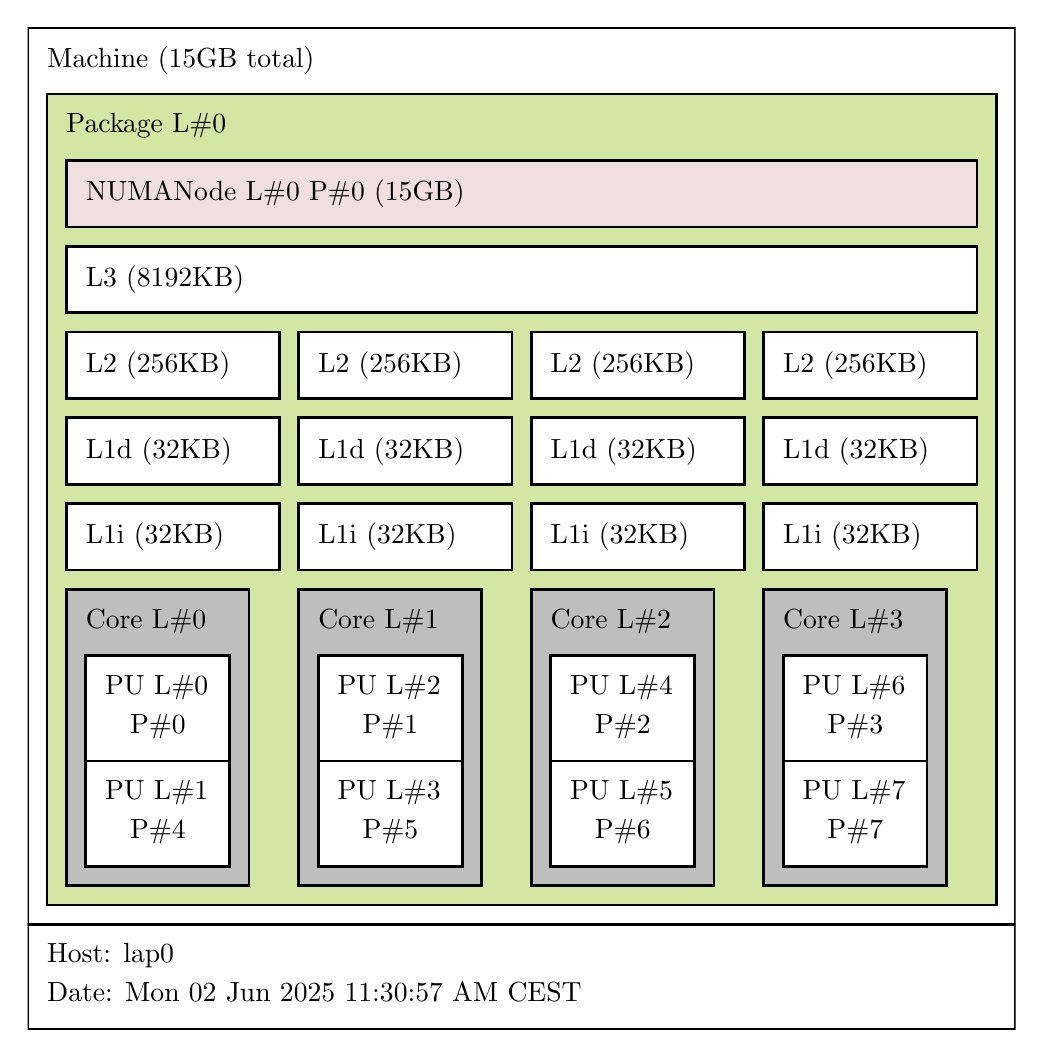
\begin{tikzpicture}[x=1pt,y=1pt,yscale=-1,hwloc-label/.style={fill=none,draw=none,text=black,align=left,anchor=north west,outer sep=0pt,inner sep=0pt,font=\fontsize{10}{14}\selectfont},hwloc-label-bold/.style={hwloc-label,font=\fontsize{10}{14}\selectfont\bfseries}]
	\clip (0,0) rectangle (357,362);
	\filldraw [fill=hwloc-color-255-255-255,draw=black,line width=1pt,solid] (0,0) rectangle ++(357,324);
	\node [hwloc-label,text=hwloc-color-0-0-0] at (7,7) {Machine (15GB total)};
	\filldraw [fill=hwloc-color-210-231-164,draw=black,line width=1pt,solid] (7,24) rectangle ++(343,293);
	\node [hwloc-label,text=hwloc-color-0-0-0] at (14,31) {Package L\#0};
	\filldraw [fill=hwloc-color-255-255-255,draw=black,line width=1pt,solid] (14,79) rectangle ++(329,24);
	\node [hwloc-label,text=hwloc-color-0-0-0] at (21,86) {L3 (8192KB)};
	\filldraw [fill=hwloc-color-255-255-255,draw=black,line width=1pt,solid] (14,110) rectangle ++(77,24);
	\node [hwloc-label,text=hwloc-color-0-0-0] at (21,117) {L2 (256KB)};
	\filldraw [fill=hwloc-color-255-255-255,draw=black,line width=1pt,solid] (14,141) rectangle ++(77,24);
	\node [hwloc-label,text=hwloc-color-0-0-0] at (21,148) {L1d (32KB)};
	\filldraw [fill=hwloc-color-255-255-255,draw=black,line width=1pt,solid] (14,172) rectangle ++(77,24);
	\node [hwloc-label,text=hwloc-color-0-0-0] at (21,179) {L1i (32KB)};
	\filldraw [fill=hwloc-color-190-190-190,draw=black,line width=1pt,solid] (14,203) rectangle ++(66,107);
	\node [hwloc-label,text=hwloc-color-0-0-0] at (21,210) {Core L\#0};
	\filldraw [fill=hwloc-color-255-255-255,draw=black,line width=1pt,solid] (21,227) rectangle ++(52,38);
	\node [hwloc-label,text=hwloc-color-0-0-0] at (28,234) {PU L\#0};
	\node [hwloc-label,text=hwloc-color-0-0-0] at (37,248) {P\#0};
	\filldraw [fill=hwloc-color-255-255-255,draw=black,line width=1pt,solid] (21,265) rectangle ++(52,38);
	\node [hwloc-label,text=hwloc-color-0-0-0] at (28,272) {PU L\#1};
	\node [hwloc-label,text=hwloc-color-0-0-0] at (37,286) {P\#4};
	\filldraw [fill=hwloc-color-255-255-255,draw=black,line width=1pt,solid] (98,110) rectangle ++(77,24);
	\node [hwloc-label,text=hwloc-color-0-0-0] at (105,117) {L2 (256KB)};
	\filldraw [fill=hwloc-color-255-255-255,draw=black,line width=1pt,solid] (98,141) rectangle ++(77,24);
	\node [hwloc-label,text=hwloc-color-0-0-0] at (105,148) {L1d (32KB)};
	\filldraw [fill=hwloc-color-255-255-255,draw=black,line width=1pt,solid] (98,172) rectangle ++(77,24);
	\node [hwloc-label,text=hwloc-color-0-0-0] at (105,179) {L1i (32KB)};
	\filldraw [fill=hwloc-color-190-190-190,draw=black,line width=1pt,solid] (98,203) rectangle ++(66,107);
	\node [hwloc-label,text=hwloc-color-0-0-0] at (105,210) {Core L\#1};
	\filldraw [fill=hwloc-color-255-255-255,draw=black,line width=1pt,solid] (105,227) rectangle ++(52,38);
	\node [hwloc-label,text=hwloc-color-0-0-0] at (112,234) {PU L\#2};
	\node [hwloc-label,text=hwloc-color-0-0-0] at (121,248) {P\#1};
	\filldraw [fill=hwloc-color-255-255-255,draw=black,line width=1pt,solid] (105,265) rectangle ++(52,38);
	\node [hwloc-label,text=hwloc-color-0-0-0] at (112,272) {PU L\#3};
	\node [hwloc-label,text=hwloc-color-0-0-0] at (121,286) {P\#5};
	\filldraw [fill=hwloc-color-255-255-255,draw=black,line width=1pt,solid] (182,110) rectangle ++(77,24);
	\node [hwloc-label,text=hwloc-color-0-0-0] at (189,117) {L2 (256KB)};
	\filldraw [fill=hwloc-color-255-255-255,draw=black,line width=1pt,solid] (182,141) rectangle ++(77,24);
	\node [hwloc-label,text=hwloc-color-0-0-0] at (189,148) {L1d (32KB)};
	\filldraw [fill=hwloc-color-255-255-255,draw=black,line width=1pt,solid] (182,172) rectangle ++(77,24);
	\node [hwloc-label,text=hwloc-color-0-0-0] at (189,179) {L1i (32KB)};
	\filldraw [fill=hwloc-color-190-190-190,draw=black,line width=1pt,solid] (182,203) rectangle ++(66,107);
	\node [hwloc-label,text=hwloc-color-0-0-0] at (189,210) {Core L\#2};
	\filldraw [fill=hwloc-color-255-255-255,draw=black,line width=1pt,solid] (189,227) rectangle ++(52,38);
	\node [hwloc-label,text=hwloc-color-0-0-0] at (196,234) {PU L\#4};
	\node [hwloc-label,text=hwloc-color-0-0-0] at (205,248) {P\#2};
	\filldraw [fill=hwloc-color-255-255-255,draw=black,line width=1pt,solid] (189,265) rectangle ++(52,38);
	\node [hwloc-label,text=hwloc-color-0-0-0] at (196,272) {PU L\#5};
	\node [hwloc-label,text=hwloc-color-0-0-0] at (205,286) {P\#6};
	\filldraw [fill=hwloc-color-255-255-255,draw=black,line width=1pt,solid] (266,110) rectangle ++(77,24);
	\node [hwloc-label,text=hwloc-color-0-0-0] at (273,117) {L2 (256KB)};
	\filldraw [fill=hwloc-color-255-255-255,draw=black,line width=1pt,solid] (266,141) rectangle ++(77,24);
	\node [hwloc-label,text=hwloc-color-0-0-0] at (273,148) {L1d (32KB)};
	\filldraw [fill=hwloc-color-255-255-255,draw=black,line width=1pt,solid] (266,172) rectangle ++(77,24);
	\node [hwloc-label,text=hwloc-color-0-0-0] at (273,179) {L1i (32KB)};
	\filldraw [fill=hwloc-color-190-190-190,draw=black,line width=1pt,solid] (266,203) rectangle ++(66,107);
	\node [hwloc-label,text=hwloc-color-0-0-0] at (273,210) {Core L\#3};
	\filldraw [fill=hwloc-color-255-255-255,draw=black,line width=1pt,solid] (273,227) rectangle ++(52,38);
	\node [hwloc-label,text=hwloc-color-0-0-0] at (280,234) {PU L\#6};
	\node [hwloc-label,text=hwloc-color-0-0-0] at (289,248) {P\#3};
	\filldraw [fill=hwloc-color-255-255-255,draw=black,line width=1pt,solid] (273,265) rectangle ++(52,38);
	\node [hwloc-label,text=hwloc-color-0-0-0] at (280,272) {PU L\#7};
	\node [hwloc-label,text=hwloc-color-0-0-0] at (289,286) {P\#7};
	\filldraw [fill=hwloc-color-239-223-222,draw=black,line width=1pt,solid] (14,48) rectangle ++(329,24);
	\node [hwloc-label,text=hwloc-color-0-0-0] at (21,55) {NUMANode L\#0 P\#0 (15GB)};
	\filldraw [fill=hwloc-color-255-255-255,draw=black,line width=1pt,solid] (0,324) rectangle ++(357,38);
	\node [hwloc-label,text=hwloc-color-0-0-0] at (7,331) {Host: lap0};
	\node [hwloc-label,text=hwloc-color-0-0-0] at (7,345) {Date: Mon 02 Jun 2025 11:30:57 AM CEST};
\end{tikzpicture}


}
  \caption[Testbed Memory Hierarchy]{The available testbed memory hierarchy. The four cores have to share the  8MB of available L3 cache.}
  \label{fig:topo}
\end{figure}

\section{Results}
\label{sec:res}
In this section, we will compare the different implementations in terms of cache-friendliness, branch predictability, and overall performance. We only consider the query phase of the implementations and not the overhead to build the trees (\texttt{"measure\_construction": false}). Since we encountered the if-conversion compiler optimization for the three-level prefetching implementation introduced in section~\ref{sec:tree} and further explained in section~\ref{subsec:pred}, we will use the compiler flags \texttt{-fno-if-conversion} and \texttt{-fno-if-conversion2} to generate a comparable binary for the standard three-level implementation reported as \texttt{BST\_EYT\_PREF\_THREE}. However, we still include the if-converted variant as \texttt{BST\_EYT\_PREF\_THREE\_IFC}. The probability-biased prefetching implementation (\texttt{BST\_EYT\_PREF\_PROB }) uses a total budget of eight prefetches. In figure \ref{fig:nspsearch} we can see the average nanoseconds taken for one execution of the \texttt{contains} function of the different implementations depending on the number of nodes. Most of the variants take between one and two hundred nanoseconds whereas the most aggressive four-level prefetching implementation (\texttt{BST\_EYT\_PREF\_FOUR}) takes around four hundred nanoseconds more on average. This is likely due to the huge pressure on the cache generated by prefetching large amounts of memory lines. We can see that the plain Eytzinger implementation (\texttt{BST\_EYT}) delivers the best performance for small instance sizes of one to three million nodes. After that, single-prefetch (\texttt{BST\_EYT\_PREF}) and if-converted three-level prefetch variants become faster. A possible explanation for this could be that the cost for the additional index calculations for prefetching may amortize for larger instances. In addition to that, the single-prefetch variant likely loads an adequate amount of lines to the cache when eviction becomes more likely as the total size of the tree increases and hence fills up the level three cache. We will study the evolution of cache misses and evictions in section~\ref{res:cache}. Unlike the standard three-level implementation which probably loads to many lines like other aggressive implementations, e.g. two, three, or four-level prefetch, the if-converted variant can still keep up with the single-level implementation, even though it probably suffers from memory bandwidth contention since it fetches the same amount as the standard three-level implementation. In section~\ref{sub:br} we will see why branch prediction is a possible explanation for this outcome.  
\begin{figure}[H]
  \centering
  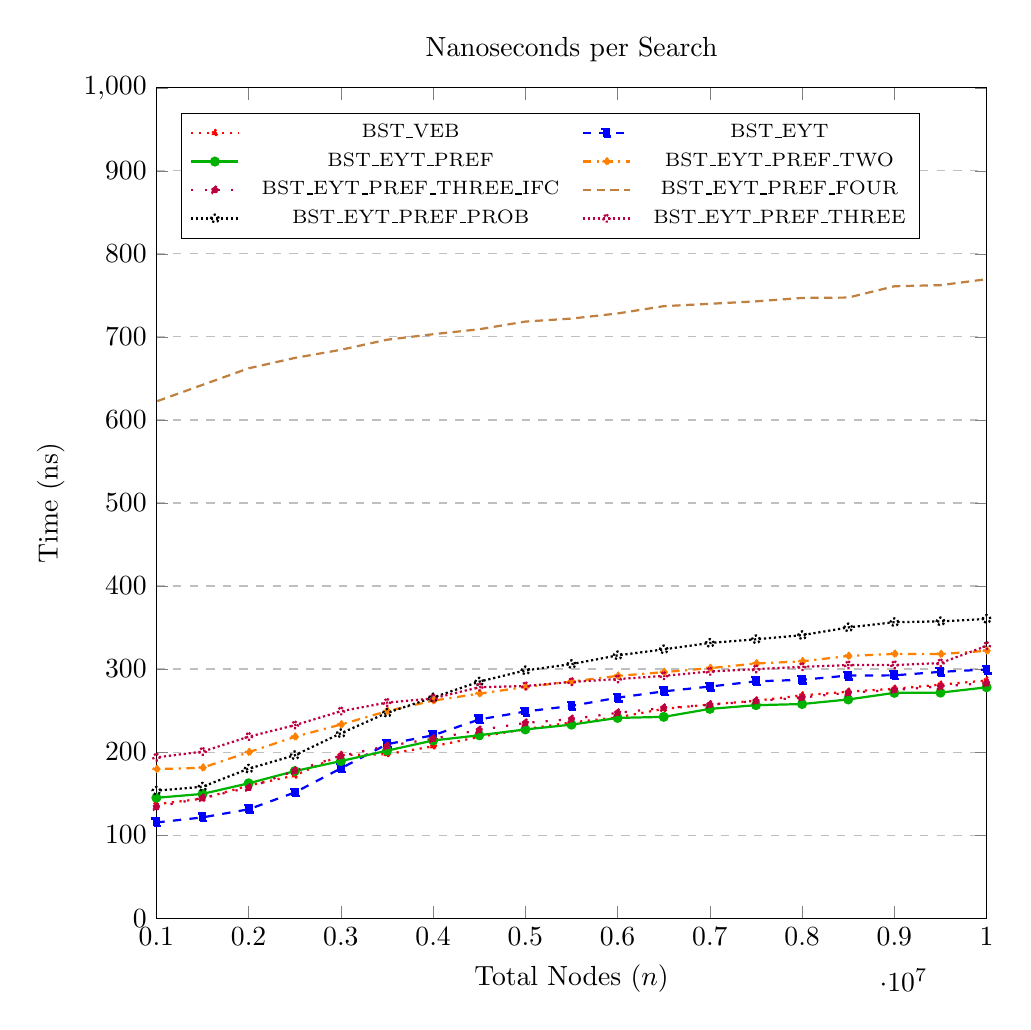
\begin{tikzpicture}
    \begin{axis}[
        title={Nanoseconds per Search},
        xlabel={Total Nodes ($n$)},
        ylabel={Time (ns)},
        width=\textwidth,
        height=1\textwidth,
        xmin=1000000, xmax=10000000,
        ymin=0, ymax=1000,
        ymajorgrids,
        grid style=dashed,
        legend columns=2,
        legend pos=north west,
        legend style={font=\scriptsize, column sep=6pt},
    ]

\addplot+[red, thick, dotted, mark=triangle*, mark options={scale=.7,fill=red}]
  coordinates {
    (500000,102.726)
    (1000000,137.13)
    (1500000,143.886)
    (2000000,159.617)
    (2500000,171.777)
    (3000000,196.365)
    (3500000,197.443)
    (4000000,206.864)
    (4500000,218.247)
    (5000000,227.587)
    (5500000,235.689)
    (6000000,241.807)
    (6500000,252.008)
    (7000000,257.294)
    (7500000,261.835)
    (8000000,268.192)
    (8500000,272.709)
    (9000000,276.222)
    (9500000,281.141)
    (10000000,286.22)
  };
\addlegendentry{BST\_VEB}

\addplot+[blue, thick, dashed, mark=square*, mark options={scale=.7,fill=blue}]
  coordinates {
    (500000,92.675)
    (1000000,115.188)
    (1500000,121.277)
    (2000000,131.068)
    (2500000,151.288)
    (3000000,180.365)
    (3500000,209.468)
    (4000000,220.168)
    (4500000,239.277)
    (5000000,248.806)
    (5500000,255.591)
    (6000000,265.492)
    (6500000,273.073)
    (7000000,278.9)
    (7500000,285.153)
    (8000000,287.066)
    (8500000,292.138)
    (9000000,292.386)
    (9500000,296.622)
    (10000000,299.403)
  };
\addlegendentry{BST\_EYT}

\addplot+[green!70!black, thick, solid, mark=*, mark options={scale=.7,fill=green!70!black}]
  coordinates {
    (500000,114.144)
    (1000000,144.896)
    (1500000,149.584)
    (2000000,162.358)
    (2500000,177.057)
    (3000000,189.114)
    (3500000,201.675)
    (4000000,213.915)
    (4500000,220.231)
    (5000000,227.221)
    (5500000,233.019)
    (6000000,241.118)
    (6500000,242.36)
    (7000000,252.003)
    (7500000,256.477)
    (8000000,257.834)
    (8500000,263.357)
    (9000000,271.258)
    (9500000,271.583)
    (10000000,278.004)
  };
\addlegendentry{BST\_EYT\_PREF}

\addplot+[orange, thick, dashdotted, mark=diamond*, mark options={scale=.7,fill=orange}]
  coordinates {
    (500000,140.616)
    (1000000,179.446)
    (1500000,181.092)
    (2000000,199.792)
    (2500000,218.321)
    (3000000,233.176)
    (3500000,249.186)
    (4000000,261.884)
    (4500000,270.372)
    (5000000,278.299)
    (5500000,284.965)
    (6000000,291.716)
    (6500000,296.259)
    (7000000,301.062)
    (7500000,306.649)
    (8000000,309.25)
    (8500000,315.71)
    (9000000,318.235)
    (9500000,317.96)
    (10000000,321.966)
  };
\addlegendentry{BST\_EYT\_PREF\_TWO}

\addplot+[purple, thick, loosely dotted, mark=pentagon*, mark options={scale=.7,fill=purple}]
  coordinates {
    (500000,104.743)
    (1000000,133.899)
    (1500000,144.771)
    (2000000,157.02)
    (2500000,177.389)
    (3000000,195.294)
    (3500000,207.233)
    (4000000,215.992)
    (4500000,226.521)
    (5000000,235.098)
    (5500000,239.645)
    (6000000,247.259)
    (6500000,253.145)
    (7000000,256.917)
    (7500000,261.485)
    (8000000,265.658)
    (8500000,271.4)
    (9000000,274.776)
    (9500000,279.107)
    (10000000,282.98)
  };
\addlegendentry{BST\_EYT\_PREF\_THREE\_IFC}

\addplot+[brown, thick, densely dashed, mark=x*, mark options={scale=.7,fill=brown}]
  coordinates {
    (500000,520.997)
    (1000000,622.281)
    (1500000,642.272)
    (2000000,662.231)
    (2500000,674.684)
    (3000000,684.506)
    (3500000,696.65)
    (4000000,703.277)
    (4500000,709.252)
    (5000000,718.52)
    (5500000,722.122)
    (6000000,728.272)
    (6500000,737.057)
    (7000000,739.914)
    (7500000,742.858)
    (8000000,746.992)
    (8500000,747.414)
    (9000000,761.055)
    (9500000,762.346)
    (10000000,769.524)
  };
\addlegendentry{BST\_EYT\_PREF\_FOUR}

\addplot+[black, thick, densely dotted, mark=o, mark options={scale=.7,fill=black}]
  coordinates {
    (500000,147.275)
    (1000000,153.474)
    (1500000,158.197)
    (2000000,179.932)
    (2500000,196.111)
    (3000000,222.617)
    (3500000,247.246)
    (4000000,265.668)
    (4500000,284.784)
    (5000000,298.337)
    (5500000,305.913)
    (6000000,316.443)
    (6500000,323.66)
    (7000000,331.411)
    (7500000,335.81)
    (8000000,340.752)
    (8500000,350.089)
    (9000000,356.393)
    (9500000,357.411)
    (10000000,360.339)
  };
\addlegendentry{BST\_EYT\_PREF\_PROB}

\addplot+[purple, thick, densely dotted, mark=pentagon, mark options={scale=.7,fill=purple}]
  coordinates {
    (500000,181.189)
    (1000000,193.529)
    (1500000,200.55)
    (2000000,218.474)
    (2500000,232.343)
    (3000000,249.176)
    (3500000,259.572)
    (4000000,264.605)
    (4500000,278.065)
    (5000000,279.55)
    (5500000,284.455)
    (6000000,287.871)
    (6500000,291.725)
    (7000000,297.017)
    (7500000,299.824)
    (8000000,302.665)
    (8500000,304.736)
    (9000000,304.825)
    (9500000,307.16)
    (10000000,327.856)
  };
\addlegendentry{BST\_EYT\_PREF\_THREE}
    \end{axis}
  \end{tikzpicture}
  \caption[Average Nanoseconds per Search of different Implementations]{Average Nanoseconds per Search (\texttt{contains()}) for the different implementations. We do not take into account the time take to build the respective trees and we always run $q=1000000$ lookups.}
  \label{fig:nspsearch}
\end{figure}


\subsection{Cache}
\label{res:cache}
In this section, we will compare the implementations regarding their locality properties. In figure~\ref{fig:cachemissbig}, we see the overall miss rates of the different versions as a function of $n$ nodes in the tree. We can observe a clear separation between the VanEmbden-Boas implementation (\texttt{BST\_VEB}) and the Eytzinger-based versions. The miss rate of the VEB layout lifts off much earlier and causes a significantly worse miss rate for larger tree sizes. The Eytzinger implementations all maintain a moderate 20-30\% miss rate and the aggressive four-level-prefetch variant can even maintain a rate below below twenty percent. The benefit of the Eytzinger layout becomes clear if we compare the plain implementation to the ones that employ manual prefetching. The layout is so predictable for the CPU-internal prefetchers that all implementations up to three levels of preloading result in comparable miss rates. This is a strong hint that in the case of the Eytzinger layout the microarchitecture of the given CPU gives us most of the benefit of prefetching for free without the need for manual programming. However, the lowest miss rate was still achieved by the four-level implementation, yet, we saw that the overall pressure of loading whole areas of the tree into the cache greatly affects performance, as reported previously in figure \ref{fig:nspsearch}. 
\begin{figure}[H]
  \centering
  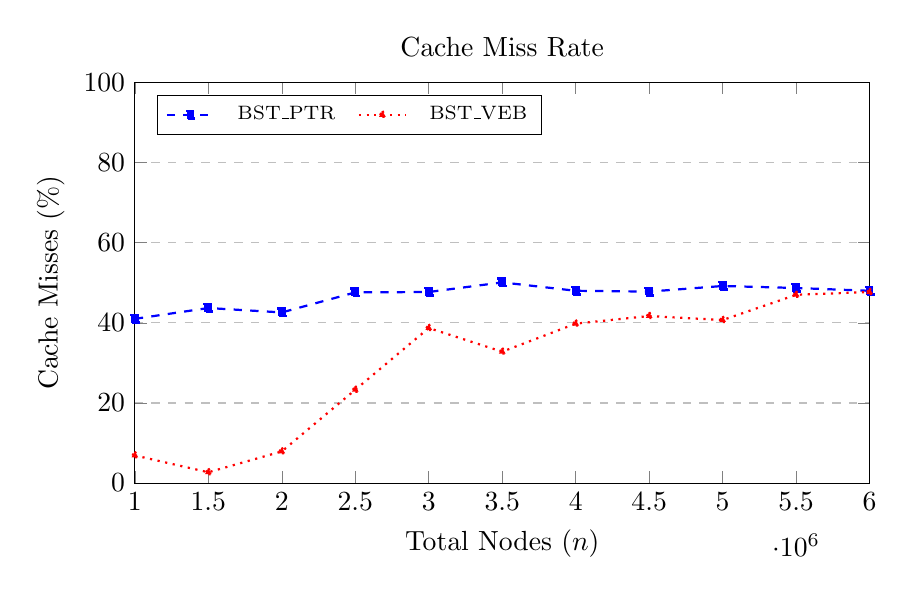
\begin{tikzpicture}
    \begin{axis}[
        title={Cache Miss Rate},
        xlabel={Total Nodes ($n$)},
        ylabel={Cache Misses (\%)},
        width=0.9\textwidth,
        height=0.55\textwidth,
        xmin=1000000, xmax=6000000,
        ymin=0, ymax=100,
        ymajorgrids,
        grid style=dashed,
        legend columns=2,
        legend pos=north west,
        legend style={font=\scriptsize, column sep=6pt},
    ]

    \addplot+[blue, thick, dashed, mark=square*, mark options={scale=.7,fill=blue}]
      coordinates {
        (1000000,41.0) (1500000,43.7) (2000000,42.6) (2500000,47.6)
        (3000000,47.7) (3500000,50.1) (4000000,48.0) (4500000,47.8)
        (5000000,49.2) (5500000,48.7) (6000000,48.0)
      };
    \addlegendentry{BST\_PTR}

    \addplot+[red, thick, dotted, mark=triangle*, mark options={scale=.7,fill=red}]
      coordinates {
        (1000000,6.9) (1500000,2.7) (2000000,7.9) (2500000,23.3)
        (3000000,38.7) (3500000,32.8) (4000000,39.8) (4500000,41.7)
        (5000000,40.7) (5500000,47.0) (6000000,47.7)
      };
    \addlegendentry{BST\_VEB}

    \end{axis}
  \end{tikzpicture}
  \caption{Cache miss rate (\%) as a function of total nodes and lookups ($q=1000000$) for the pointer-based (\texttt{BST\_PTR}) and VanEmde-Boas (\texttt{BST\_VEB}) implementations.}
  \label{fig:cachemissbig}
\end{figure}


The level-one miss rate seen in figure~\ref{fig:l1miss} reveals a different outcome from the total miss results. If we only consider the level-one miss rate, the plain Eytzinger version has to go to higher memory levels significantly more often followed by the VEB implementation. Depending on how aggressively we prefetch an area of the tree, the fewer misses we will cause. Untimely, the four-level version is constantly overwriting large parts of the cache with the area that is currently queried which results in a low miss rate, but high contention and hence negative performance impact.  
\begin{figure}[H]
  \centering
  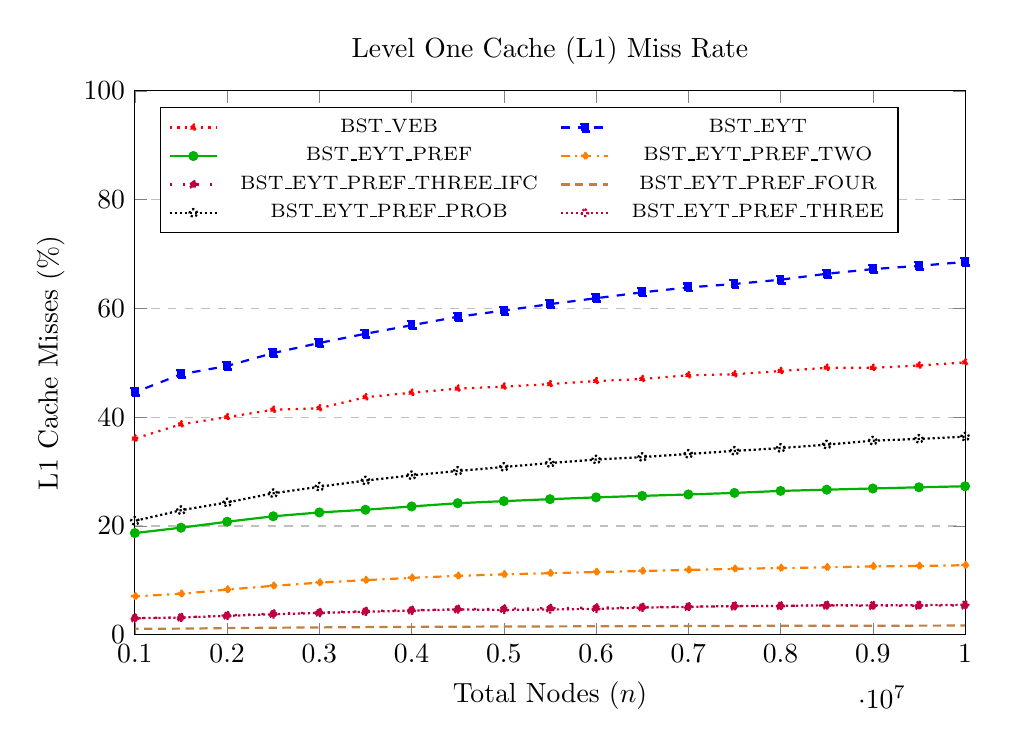
\begin{tikzpicture}
    \begin{axis}[
        title={Level One Cache (L1) Miss Rate},
        xlabel={Total Nodes ($n$)},
        ylabel={L1 Cache Misses (\%)},
        width=\textwidth,
        height=0.7\textwidth,
        xmin=1000000, xmax=10000000,
        ymin=0, ymax=100,
        ymajorgrids,
        grid style=dashed,
        legend columns=2,
        legend pos=north west,
        legend style={font=\scriptsize, column sep=6pt},
    ]
\addplot+[red, thick, dotted, mark=triangle*, mark options={scale=.7,fill=red}]
  coordinates {
    (500000,31.3062)
    (1000000,36.0758)
    (1500000,38.6957)
    (2000000,40.013)
    (2500000,41.3807)
    (3000000,41.6471)
    (3500000,43.6703)
    (4000000,44.5051)
    (4500000,45.2573)
    (5000000,45.6278)
    (5500000,46.0871)
    (6000000,46.6518)
    (6500000,47.0213)
    (7000000,47.7234)
    (7500000,47.8965)
    (8000000,48.497)
    (8500000,49.0978)
    (9000000,49.0774)
    (9500000,49.5094)
    (10000000,50.0791)
  };
\addlegendentry{BST\_VEB}

\addplot+[blue, thick, dashed, mark=square*, mark options={scale=.7,fill=blue}]
  coordinates {
    (500000,39.0021)
    (1000000,44.5877)
    (1500000,47.8964)
    (2000000,49.4251)
    (2500000,51.8032)
    (3000000,53.6561)
    (3500000,55.352)
    (4000000,56.9129)
    (4500000,58.4679)
    (5000000,59.618)
    (5500000,60.7986)
    (6000000,61.8838)
    (6500000,62.9677)
    (7000000,63.8708)
    (7500000,64.4956)
    (8000000,65.2909)
    (8500000,66.3802)
    (9000000,67.2387)
    (9500000,67.8398)
    (10000000,68.5556)
  };
\addlegendentry{BST\_EYT}

\addplot+[green!70!black, thick, solid, mark=*, mark options={scale=.7,fill=green!70!black}]
  coordinates {
    (500000,16.9211)
    (1000000,18.7014)
    (1500000,19.6844)
    (2000000,20.7806)
    (2500000,21.7831)
    (3000000,22.4891)
    (3500000,22.9833)
    (4000000,23.5898)
    (4500000,24.1884)
    (5000000,24.5703)
    (5500000,24.9296)
    (6000000,25.2622)
    (6500000,25.5371)
    (7000000,25.7949)
    (7500000,26.0831)
    (8000000,26.451)
    (8500000,26.6761)
    (9000000,26.8954)
    (9500000,27.1143)
    (10000000,27.3047)
  };
\addlegendentry{BST\_EYT\_PREF}

\addplot+[orange, thick, dashdotted, mark=diamond*, mark options={scale=.7,fill=orange}]
  coordinates {
    (500000,6.20913)
    (1000000,7.06607)
    (1500000,7.5222)
    (2000000,8.30271)
    (2500000,8.99257)
    (3000000,9.58598)
    (3500000,10.0427)
    (4000000,10.4562)
    (4500000,10.833)
    (5000000,11.1054)
    (5500000,11.3116)
    (6000000,11.5295)
    (6500000,11.7147)
    (7000000,11.9128)
    (7500000,12.128)
    (8000000,12.2579)
    (8500000,12.3976)
    (9000000,12.5729)
    (9500000,12.6419)
    (10000000,12.7869)
  };
\addlegendentry{BST\_EYT\_PREF\_TWO}

\addplot+[purple, thick, loosely dotted, mark=pentagon*, mark options={scale=.7,fill=purple}]
  coordinates {
    (500000,2.79783)
    (1000000,3.05486)
    (1500000,3.18267)
    (2000000,3.55698)
    (2500000,3.87104)
    (3000000,4.10848)
    (3500000,4.32593)
    (4000000,4.51679)
    (4500000,4.68658)
    (5000000,4.78276)
    (5500000,4.8809)
    (6000000,4.97628)
    (6500000,5.07373)
    (7000000,5.15563)
    (7500000,5.22983)
    (8000000,5.30515)
    (8500000,5.39602)
    (9000000,5.29358)
    (9500000,5.33681)
    (10000000,5.38145)
  };
\addlegendentry{BST\_EYT\_PREF\_THREE\_IFC}

\addplot+[brown, thick, densely dashed, mark=x*, mark options={scale=.7,fill=brown}]
  coordinates {
    (500000,0.994834)
    (1000000,1.08558)
    (1500000,1.12831)
    (2000000,1.21473)
    (2500000,1.29196)
    (3000000,1.34979)
    (3500000,1.40276)
    (4000000,1.44409)
    (4500000,1.48085)
    (5000000,1.50931)
    (5500000,1.52937)
    (6000000,1.5612)
    (6500000,1.58161)
    (7000000,1.5988)
    (7500000,1.62005)
    (8000000,1.6456)
    (8500000,1.66216)
    (9000000,1.66317)
    (9500000,1.67409)
    (10000000,1.68647)
  };
\addlegendentry{BST\_EYT\_PREF\_FOUR}

\addplot+[black, thick, densely dotted, mark=o, mark options={scale=.7,fill=black}]
  coordinates {
    (500000,18.0054)
    (1000000,20.9407)
    (1500000,22.8932)
    (2000000,24.3216)
    (2500000,26.012)
    (3000000,27.2179)
    (3500000,28.3479)
    (4000000,29.3114)
    (4500000,30.1139)
    (5000000,30.8506)
    (5500000,31.5713)
    (6000000,32.2155)
    (6500000,32.6706)
    (7000000,33.2423)
    (7500000,33.8017)
    (8000000,34.326)
    (8500000,34.954)
    (9000000,35.685)
    (9500000,36.0124)
    (10000000,36.4359)
  };
\addlegendentry{BST\_EYT\_PREF\_PROB}

\addplot+[purple, thick, densely dotted, mark=pentagon, mark options={scale=.7,fill=purple}]
  coordinates {
    (500000,2.78606)
    (1000000,3.03333)
    (1500000,3.16082)
    (2000000,3.47135)
    (2500000,3.76325)
    (3000000,4.00419)
    (3500000,4.23065)
    (4000000,4.43485)
    (4500000,4.64675)
    (5000000,4.55443)
    (5500000,4.64449)
    (6000000,4.75418)
    (6500000,4.98362)
    (7000000,5.13598)
    (7500000,5.28373)
    (8000000,5.30827)
    (8500000,5.41954)
    (9000000,5.39481)
    (9500000,5.44417)
    (10000000,5.5058)
  };
\addlegendentry{BST\_EYT\_PREF\_THREE}

    \end{axis}
  \end{tikzpicture}
  \caption[L1 Cache Miss Rate]{L1 Cache miss rate for the different implementations.}
  \label{fig:l1miss}
\end{figure}


In figure~\ref{fig:l3miss}, we can see how we can utilize the L3 cache more aggressively by employing manual prefetching. Because of its larger size, we can fit larger areas of the tree into fast cache memory and reduce the miss rate, even if we mostly fetch useless lines with respect to the current query. If we compare the nanoseconds taken from figure~\ref{fig:nspsearch} with the L3 cache miss rate, we can conclude that a moderate two to three-level prefetch is a good balance between enhanced locality and contention on the memory system. 
\begin{figure}[H]
  \centering
  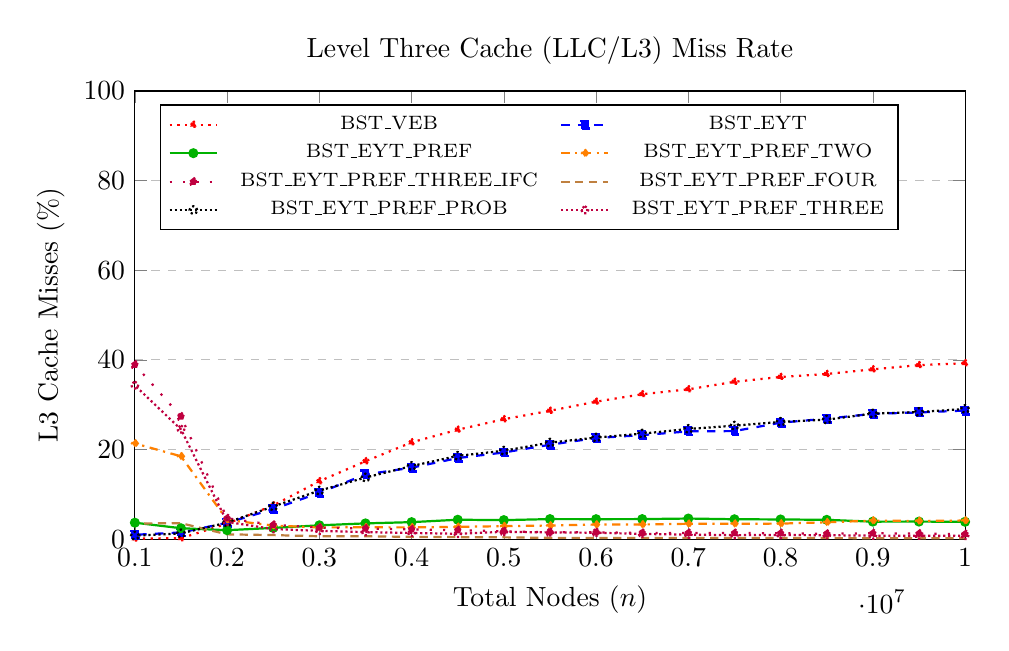
\begin{tikzpicture}
    \begin{axis}[
        title={Level Three Cache (LLC/L3) Miss Rate},
        xlabel={Total Nodes ($n$)},
        ylabel={L3 Cache Misses (\%)},
        width=\textwidth,
        height=0.6\textwidth,
        xmin=1000000, xmax=10000000,
        ymin=0, ymax=100,
        ymajorgrids,
        grid style=dashed,
        legend columns=2,
        legend pos=north west,
        legend style={font=\scriptsize, column sep=6pt},
    ]

\addplot+[red, thick, dotted, mark=triangle*, mark options={scale=.7,fill=red}]
  coordinates {
    (500000,0.174708)
    (1000000,0.172303)
    (1500000,0.230831)
    (2000000,3.48297)
    (2500000,7.54405)
    (3000000,12.9524)
    (3500000,17.3906)
    (4000000,21.6216)
    (4500000,24.4402)
    (5000000,26.7795)
    (5500000,28.6673)
    (6000000,30.6915)
    (6500000,32.3606)
    (7000000,33.4494)
    (7500000,35.1244)
    (8000000,36.2091)
    (8500000,36.8686)
    (9000000,37.9049)
    (9500000,38.8461)
    (10000000,39.2651)
  };
\addlegendentry{BST\_VEB}

\addplot+[blue, thick, dashed, mark=square*, mark options={scale=.7,fill=blue}]
  coordinates {
    (500000,0.24494)
    (1000000,1.00856)
    (1500000,1.51786)
    (2000000,3.66238)
    (2500000,6.71936)
    (3000000,10.3579)
    (3500000,14.4584)
    (4000000,15.9637)
    (4500000,18.1108)
    (5000000,19.3566)
    (5500000,21.0839)
    (6000000,22.5908)
    (6500000,23.23)
    (7000000,24.0674)
    (7500000,24.1319)
    (8000000,26.0098)
    (8500000,26.8975)
    (9000000,27.9818)
    (9500000,28.2901)
    (10000000,28.7109)
  };
\addlegendentry{BST\_EYT}

\addplot+[green!70!black, thick, solid, mark=*, mark options={scale=.7,fill=green!70!black}]
  coordinates {
    (500000,5.91621)
    (1000000,3.7)
    (1500000,2.46281)
    (2000000,2.02618)
    (2500000,2.53364)
    (3000000,3.11245)
    (3500000,3.54562)
    (4000000,3.82068)
    (4500000,4.35903)
    (5000000,4.27307)
    (5500000,4.50095)
    (6000000,4.48439)
    (6500000,4.50154)
    (7000000,4.62524)
    (7500000,4.46707)
    (8000000,4.42205)
    (8500000,4.33766)
    (9000000,3.92995)
    (9500000,3.94563)
    (10000000,3.89844)
  };
\addlegendentry{BST\_EYT\_PREF}

\addplot+[orange, thick, dashdotted, mark=diamond*, mark options={scale=.7,fill=orange}]
  coordinates {
    (500000,25.3308)
    (1000000,21.3796)
    (1500000,18.5081)
    (2000000,4.33598)
    (2500000,3.04895)
    (3000000,2.65075)
    (3500000,2.66488)
    (4000000,2.65196)
    (4500000,2.76563)
    (5000000,2.92698)
    (5500000,3.06885)
    (6000000,3.28907)
    (6500000,3.30572)
    (7000000,3.45214)
    (7500000,3.46997)
    (8000000,3.49213)
    (8500000,3.79129)
    (9000000,4.1608)
    (9500000,4.08711)
    (10000000,4.17599)
  };
\addlegendentry{BST\_EYT\_PREF\_TWO}

\addplot+[purple, thick, loosely dotted, mark=pentagon*, mark options={scale=.7,fill=purple}]
  coordinates {
    (500000,45.2258)
    (1000000,38.9509)
    (1500000,27.3737)
    (2000000,4.68237)
    (2500000,3.21968)
    (3000000,2.60981)
    (3500000,2.41296)
    (4000000,2.21701)
    (4500000,2.01558)
    (5000000,1.78265)
    (5500000,1.56477)
    (6000000,1.55039)
    (6500000,1.412)
    (7000000,1.3981)
    (7500000,1.39432)
    (8000000,1.34351)
    (8500000,1.22791)
    (9000000,1.3402)
    (9500000,1.26456)
    (10000000,1.15623)
  };
\addlegendentry{BST\_EYT\_PREF\_THREE\_IFC}

\addplot+[brown, thick, densely dashed, mark=x*, mark options={scale=.7,fill=brown}]
  coordinates {
    (500000,3.77829)
    (1000000,3.52375)
    (1500000,3.58718)
    (2000000,1.09697)
    (2500000,0.933498)
    (3000000,0.671307)
    (3500000,0.669338)
    (4000000,0.533449)
    (4500000,0.474147)
    (5000000,0.430299)
    (5500000,0.314069)
    (6000000,0.306923)
    (6500000,0.312449)
    (7000000,0.306653)
    (7500000,0.280463)
    (8000000,0.267104)
    (8500000,0.264681)
    (9000000,0.242956)
    (9500000,0.240664)
    (10000000,0.233908)
  };
\addlegendentry{BST\_EYT\_PREF\_FOUR}

\addplot+[black, thick, densely dotted, mark=o, mark options={scale=.7,fill=black}]
  coordinates {
    (500000,0.202921)
    (1000000,0.809497)
    (1500000,1.31423)
    (2000000,3.71704)
    (2500000,7.31368)
    (3000000,10.8502)
    (3500000,13.7684)
    (4000000,16.3302)
    (4500000,18.6039)
    (5000000,19.7459)
    (5500000,21.557)
    (6000000,22.6796)
    (6500000,23.5631)
    (7000000,24.6014)
    (7500000,25.339)
    (8000000,26.1779)
    (8500000,26.6729)
    (9000000,28.0361)
    (9500000,28.3843)
    (10000000,29.0648)
  };
\addlegendentry{BST\_EYT\_PREF\_PROB}

\addplot+[purple, thick, densely dotted, mark=pentagon, mark options={scale=.7,fill=purple}]
  coordinates {
    (500000,37.0721)
    (1000000,34.313)
    (1500000,24.5053)
    (2000000,3.86644)
    (2500000,2.28511)
    (3000000,1.87441)
    (3500000,1.59834)
    (4000000,1.40515)
    (4500000,1.22843)
    (5000000,1.66556)
    (5500000,1.52754)
    (6000000,1.46442)
    (6500000,1.18309)
    (7000000,1.04515)
    (7500000,0.922377)
    (8000000,0.958146)
    (8500000,0.901874)
    (9000000,0.804803)
    (9500000,0.791203)
    (10000000,0.773964)
  };
\addlegendentry{BST\_EYT\_PREF\_THREE}
    \end{axis}
  \end{tikzpicture}
  \caption[L3 Cache Miss Rate]{L3 Cache miss rate for the different implementations.}
  \label{fig:l3miss}
\end{figure}


The plots seen in figure~\ref{fig:missperop} compare absolute numbers of full cache misses of the different implementations. In particular, we see the average number of cache misses taken per search operation. It is important to note that these misses also include those triggered by prefetching operations. Hence, the plain Eytzinger version tries to touch the least amount of lines and hence takes the least misses per search on average. Interestingly, the probabilistic implementation closely follows this trend. Once we process about eight to nine million nodes, we see a sudden increase for the four-level prefetching while the other implementations can maintain a shallow development. At this point, the aggressive prefetching may constantly have to evict important sections of the tree, e.g. the root area, upon every traversal which causes this sudden increase. The VEB implementation consistently causes the most misses per search, but also only pulls in memory lines that are actually useful for the current query. 
\begin{figure}[H]
  \centering
  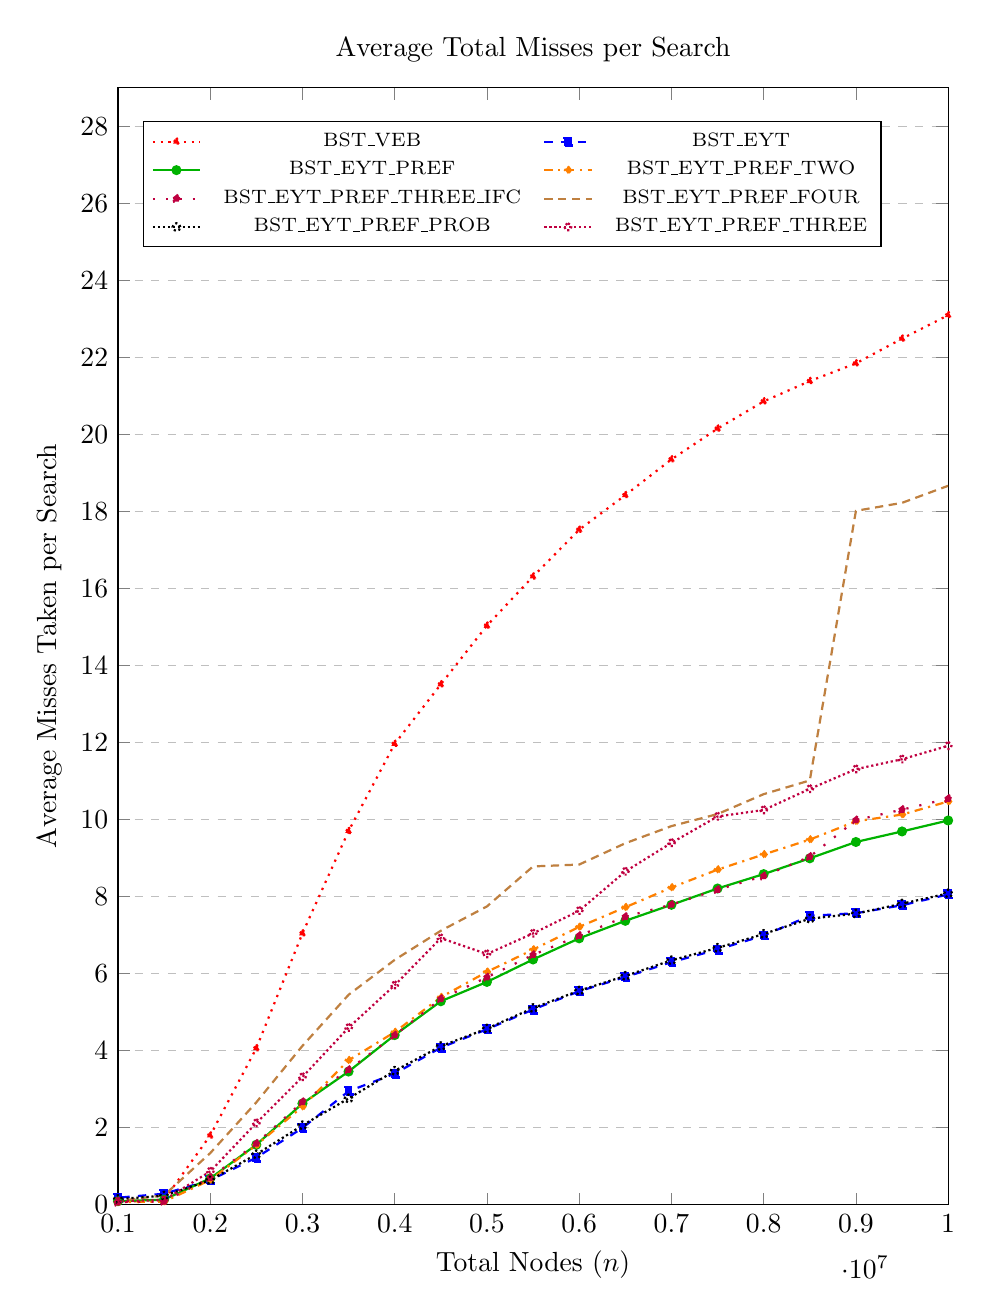
\begin{tikzpicture}
    \begin{axis}[
        title={Average Total Misses per Search},
        xlabel={Total Nodes ($n$)},
        ylabel={Average Misses Taken per Search},
        width=\textwidth,
        height=1.3\textwidth,
        xmin=1000000, xmax=10000000,
        ymin=0, ymax=29,
        ymajorgrids,
        grid style=dashed,
        legend columns=2,
        legend pos=north west,
        legend style={font=\scriptsize, column sep=6pt},
    ]
\addplot+[red, thick, dotted, mark=triangle*, mark options={scale=.7,fill=red}]
  coordinates {
    (500000,0.0548921)
    (1000000,0.0629666)
    (1500000,0.118733)
    (2000000,1.79157)
    (2500000,4.05789)
    (3000000,7.04204)
    (3500000,9.6992)
    (4000000,11.9625)
    (4500000,13.5091)
    (5000000,15.0344)
    (5500000,16.3101)
    (6000000,17.5242)
    (6500000,18.4224)
    (7000000,19.3508)
    (7500000,20.1498)
    (8000000,20.8572)
    (8500000,21.385)
    (9000000,21.8442)
    (9500000,22.487)
    (10000000,23.096)
  };
\addlegendentry{BST\_VEB}

\addplot+[blue, thick, dashed, mark=square*, mark options={scale=.7,fill=blue}]
  coordinates {
    (500000,0.0653105)
    (1000000,0.177027)
    (1500000,0.279993)
    (2000000,0.632362)
    (2500000,1.21673)
    (3000000,1.98822)
    (3500000,2.94199)
    (4000000,3.39748)
    (4500000,4.07406)
    (5000000,4.55061)
    (5500000,5.06365)
    (6000000,5.53851)
    (6500000,5.90764)
    (7000000,6.29444)
    (7500000,6.62049)
    (8000000,6.98652)
    (8500000,7.49655)
    (9000000,7.56631)
    (9500000,7.77159)
    (10000000,8.05284)
  };
\addlegendentry{BST\_EYT}

\addplot+[green!70!black, thick, solid, mark=*, mark options={scale=.7,fill=green!70!black}]
  coordinates {
    (500000,0.0686313)
    (1000000,0.086969)
    (1500000,0.126726)
    (2000000,0.678286)
    (2500000,1.5528)
    (3000000,2.62253)
    (3500000,3.45319)
    (4000000,4.40053)
    (4500000,5.27865)
    (5000000,5.78078)
    (5500000,6.36387)
    (6000000,6.91269)
    (6500000,7.3678)
    (7000000,7.78316)
    (7500000,8.20733)
    (8000000,8.58111)
    (8500000,8.99082)
    (9000000,9.41528)
    (9500000,9.68902)
    (10000000,9.97386)
  };
\addlegendentry{BST\_EYT\_PREF}

\addplot+[orange, thick, dashdotted, mark=diamond*, mark options={scale=.7,fill=orange}]
  coordinates {
    (500000,0.0547847)
    (1000000,0.062993)
    (1500000,0.074297)
    (2000000,0.637269)
    (2500000,1.54314)
    (3000000,2.54082)
    (3500000,3.74535)
    (4000000,4.47743)
    (4500000,5.38241)
    (5000000,6.04195)
    (5500000,6.62004)
    (6000000,7.21066)
    (6500000,7.71956)
    (7000000,8.23222)
    (7500000,8.69706)
    (8000000,9.09099)
    (8500000,9.47667)
    (9000000,9.95257)
    (9500000,10.1271)
    (10000000,10.4672)
  };
\addlegendentry{BST\_EYT\_PREF\_TWO}

\addplot+[purple, thick, loosely dotted, mark=pentagon*, mark options={scale=.7,fill=purple}]
  coordinates {
    (500000,0.0537039)
    (1000000,0.0583465)
    (1500000,0.0800673)
    (2000000,0.692795)
    (2500000,1.58472)
    (3000000,2.6649)
    (3500000,3.49907)
    (4000000,4.3946)
    (4500000,5.33898)
    (5000000,5.90061)
    (5500000,6.48378)
    (6000000,6.9811)
    (6500000,7.47375)
    (7000000,7.78957)
    (7500000,8.17538)
    (8000000,8.52959)
    (8500000,9.03388)
    (9000000,9.98362)
    (9500000,10.2546)
    (10000000,10.5412)
  };
\addlegendentry{BST\_EYT\_PREF\_THREE\_IFC}

\addplot+[brown, thick, densely dashed, mark=x*, mark options={scale=.7,fill=brown}]
  coordinates {
    (500000,0.0741222)
    (1000000,0.0918718)
    (1500000,0.238051)
    (2000000,1.33413)
    (2500000,2.65312)
    (3000000,4.12054)
    (3500000,5.44616)
    (4000000,6.35319)
    (4500000,7.10996)
    (5000000,7.74147)
    (5500000,8.78054)
    (6000000,8.82906)
    (6500000,9.38241)
    (7000000,9.82721)
    (7500000,10.1401)
    (8000000,10.6573)
    (8500000,11.0133)
    (9000000,18.0149)
    (9500000,18.2231)
    (10000000,18.6655)
  };
\addlegendentry{BST\_EYT\_PREF\_FOUR}

\addplot+[black, thick, densely dotted, mark=o, mark options={scale=.7,fill=black}]
  coordinates {
    (500000,0.0588608)
    (1000000,0.142059)
    (1500000,0.22839)
    (2000000,0.632855)
    (2500000,1.30175)
    (3000000,2.05558)
    (3500000,2.75447)
    (4000000,3.47087)
    (4500000,4.11114)
    (5000000,4.56843)
    (5500000,5.10093)
    (6000000,5.55407)
    (6500000,5.93604)
    (7000000,6.34128)
    (7500000,6.66369)
    (8000000,7.02534)
    (8500000,7.4237)
    (9000000,7.55398)
    (9500000,7.81251)
    (10000000,8.08041)
  };
\addlegendentry{BST\_EYT\_PREF\_PROB}

\addplot+[purple, thick, densely dotted, mark=pentagon, mark options={scale=.7,fill=purple}]
  coordinates {
    (500000,0.0596313)
    (1000000,0.0851192)
    (1500000,0.116495)
    (2000000,0.859235)
    (2500000,2.11671)
    (3000000,3.31271)
    (3500000,4.59207)
    (4000000,5.69539)
    (4500000,6.91712)
    (5000000,6.50577)
    (5500000,7.0409)
    (6000000,7.62942)
    (6500000,8.64894)
    (7000000,9.39286)
    (7500000,10.0773)
    (8000000,10.2456)
    (8500000,10.7933)
    (9000000,11.3066)
    (9500000,11.5641)
    (10000000,11.9127)
  };
\addlegendentry{BST\_EYT\_PREF\_THREE}

    \end{axis}
  \end{tikzpicture}
  \caption[Average Cache Misses Taken Per Search]{Average Cache Misses Taken Per Search for the different implementations}
  \label{fig:missperop}
\end{figure}


\subsection{Branch Prediction}
\label{sub:br}
In this section, we will report the control-flow properties and branch prediction friendliness as well as the effects of predication. We will differentiate between those branches that are easy to predict and hence have no or very little performance impact on the program and those that are basically impossible to consistently predict correctly. In figure~\ref{fig:totalbraches}, we see the total amount of branches that have to be executed for the given implementation. The more lines we want to attempt to prefetch, the more bound checks we have to perform. This is why the four-level implementation executed by far the most branches. The other implementations require near-proportionally less bound checks and hence branches. The two three-level versions are offset by a small margin, likely the branch which was if-converted. Even though the difference is very small, we can observe a massive difference in terms of branch predictability, as can be seen in figure~\ref{fig:branchrate}.
\begin{figure}[H]
  \centering
  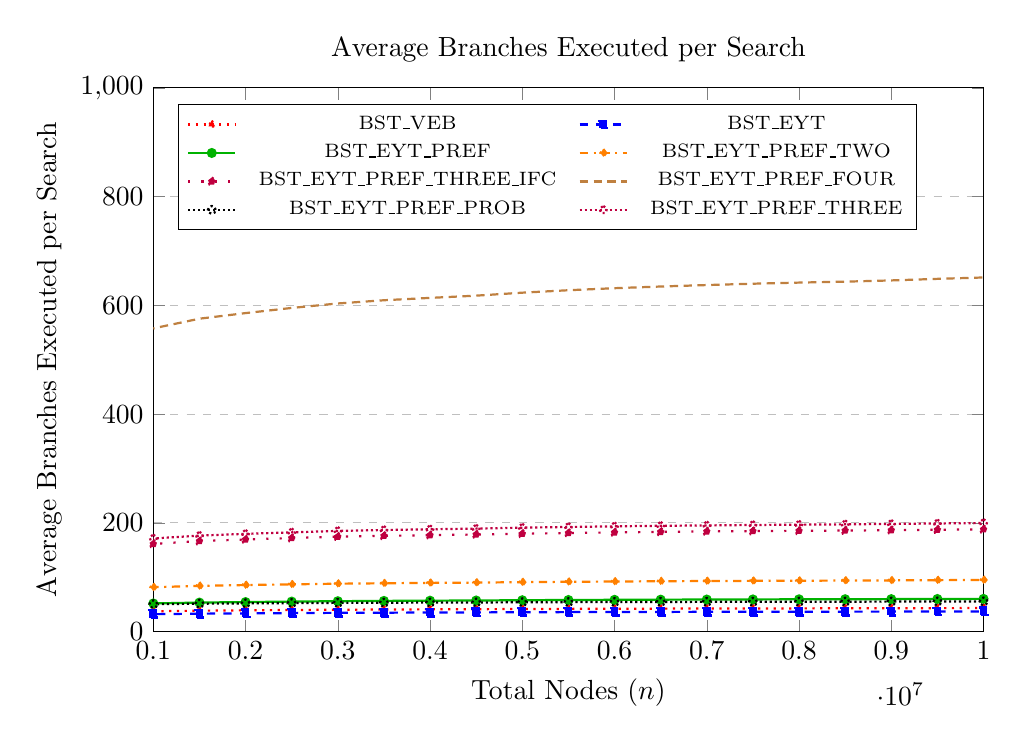
\begin{tikzpicture}
    \begin{axis}[
        title={Average Branches Executed per Search},
        xlabel={Total Nodes ($n$)},
        ylabel={Average Branches Executed per Search},
        width=\textwidth,
        height=0.7\textwidth,
        xmin=1000000, xmax=10000000,
        ymin=0, ymax=1000,
        ymajorgrids,
        grid style=dashed,
        legend columns=2,
        legend pos=north west,
        legend style={font=\scriptsize, column sep=6pt},
    ]

\addplot+[red, thick, dotted, mark=triangle*, mark options={scale=.7,fill=red}]
  coordinates {
    (500000,35.7548)
    (1000000,37.4596)
    (1500000,38.5689)
    (2000000,39.2593)
    (2500000,39.8635)
    (3000000,40.3432)
    (3500000,40.7333)
    (4000000,41.061)
    (4500000,41.3402)
    (5000000,41.6532)
    (5500000,41.9267)
    (6000000,42.1222)
    (6500000,42.3709)
    (7000000,42.5156)
    (7500000,42.6558)
    (8000000,42.8116)
    (8500000,42.9712)
    (9000000,43.076)
    (9500000,43.277)
    (10000000,43.3998)
  };
\addlegendentry{BST\_VEB}

\addplot+[blue, thick, dashed, mark=square*, mark options={scale=.7,fill=blue}]
  coordinates {
    (500000,30.6173)
    (1000000,32.1408)
    (1500000,33.0816)
    (2000000,33.6359)
    (2500000,34.1684)
    (3000000,34.6539)
    (3500000,34.9313)
    (4000000,35.1642)
    (4500000,35.4172)
    (5000000,35.7008)
    (5500000,35.9517)
    (6000000,36.1493)
    (6500000,36.3166)
    (7000000,36.4804)
    (7500000,36.6077)
    (8000000,36.714)
    (8500000,36.8003)
    (9000000,36.9136)
    (9500000,37.0841)
    (10000000,37.2201)
  };
\addlegendentry{BST\_EYT}

\addplot+[green!70!black, thick, solid, mark=*, mark options={scale=.7,fill=green!70!black}]
  coordinates {
    (500000,49.424)
    (1000000,51.9043)
    (1500000,53.4926)
    (2000000,54.4311)
    (2500000,55.3321)
    (3000000,56.0244)
    (3500000,56.5851)
    (4000000,56.9661)
    (4500000,57.3289)
    (5000000,57.8218)
    (5500000,58.2554)
    (6000000,58.5701)
    (6500000,58.845)
    (7000000,59.0827)
    (7500000,59.3068)
    (8000000,59.4954)
    (8500000,59.6695)
    (9000000,59.8461)
    (9500000,60.1188)
    (10000000,60.3164)
  };
\addlegendentry{BST\_EYT\_PREF}

\addplot+[orange, thick, dashdotted, mark=diamond*, mark options={scale=.7,fill=orange}]
  coordinates {
    (500000,77.6266)
    (1000000,81.7322)
    (1500000,84.1925)
    (2000000,85.743)
    (2500000,87.0173)
    (3000000,88.2005)
    (3500000,89.0158)
    (4000000,89.6991)
    (4500000,90.2446)
    (5000000,91.0629)
    (5500000,91.733)
    (6000000,92.2253)
    (6500000,92.7404)
    (7000000,93.0984)
    (7500000,93.4445)
    (8000000,93.6858)
    (8500000,93.9759)
    (9000000,94.3041)
    (9500000,94.7135)
    (10000000,95.0857)
  };
\addlegendentry{BST\_EYT\_PREF\_TWO}

\addplot+[purple, thick, loosely dotted, mark=pentagon*, mark options={scale=.7,fill=purple}]
  coordinates {
    (500000,153.325)
    (1000000,161.387)
    (1500000,166.517)
    (2000000,169.526)
    (2500000,172.167)
    (3000000,174.653)
    (3500000,176.172)
    (4000000,177.422)
    (4500000,178.699)
    (5000000,180.014)
    (5500000,181.433)
    (6000000,182.495)
    (6500000,183.489)
    (7000000,184.302)
    (7500000,184.946)
    (8000000,185.477)
    (8500000,185.98)
    (9000000,186.563)
    (9500000,187.415)
    (10000000,188.144)
  };
\addlegendentry{BST\_EYT\_PREF\_THREE\_IFC}

\addplot+[brown, thick, densely dashed, mark=x*, mark options={scale=.7,fill=brown}]
  coordinates {
    (500000,529.714)
    (1000000,557.707)
    (1500000,575.53)
    (2000000,585.842)
    (2500000,595.301)
    (3000000,603.515)
    (3500000,609.458)
    (4000000,613.797)
    (4500000,617.908)
    (5000000,623.381)
    (5500000,627.871)
    (6000000,631.629)
    (6500000,634.703)
    (7000000,637.393)
    (7500000,639.869)
    (8000000,641.91)
    (8500000,643.644)
    (9000000,645.915)
    (9500000,648.787)
    (10000000,651.351)
  };
\addlegendentry{BST\_EYT\_PREF\_FOUR}

\addplot+[black, thick, densely dotted, mark=o, mark options={scale=.7,fill=black}]
  coordinates {
    (500000,48.9526)
    (1000000,50.4912)
    (1500000,51.4254)
    (2000000,52.0073)
    (2500000,52.5033)
    (3000000,52.9719)
    (3500000,53.27)
    (4000000,53.5151)
    (4500000,53.73)
    (5000000,54.0084)
    (5500000,54.2906)
    (6000000,54.4819)
    (6500000,54.6435)
    (7000000,54.8052)
    (7500000,54.9357)
    (8000000,55.046)
    (8500000,55.1636)
    (9000000,55.2689)
    (9500000,55.4345)
    (10000000,55.5513)
  };
\addlegendentry{BST\_EYT\_PREF\_PROB}

\addplot+[purple, thick, densely dotted, mark=pentagon, mark options={scale=.7,fill=purple}]
  coordinates {
    (500000,162.649)
    (1000000,171.375)
    (1500000,176.616)
    (2000000,179.89)
    (2500000,182.605)
    (3000000,185.255)
    (3500000,186.945)
    (4000000,188.287)
    (4500000,189.52)
    (5000000,191.278)
    (5500000,192.511)
    (6000000,193.684)
    (6500000,194.708)
    (7000000,195.328)
    (7500000,196.181)
    (8000000,196.767)
    (8500000,197.386)
    (9000000,198.126)
    (9500000,198.99)
    (10000000,199.72)
  };
\addlegendentry{BST\_EYT\_PREF\_THREE}

    \end{axis}
  \end{tikzpicture}
  \caption[Average Branches Executed per Search]{The figure includes the average branches which have to be executed for the given implementation per search operation.}
  \label{fig:totalbraches}
\end{figure}


In fact, the if-converted three-level prefetch implementation virtually causes no mispredictions because the critical if-statement was predicated, as we saw earlier in section~\ref{subsec:pred}. For the remaining implementations, we can see how the easy-to-predict bound checks water down the miss rate. Up to this point, the three-level prefetching implementation and its if-converted version showed very similar metrics, e.g. in terms of locality. However, we saw in figure~\ref{fig:nspsearch} that the predicated version constantly delivers better performance. We can certainly relate this increase in performance to the fact that the predicated version does not suffer from hard-to-predict branches and the resulting performance penalty of branch misprediction. 
\begin{figure}[H]
  \centering
  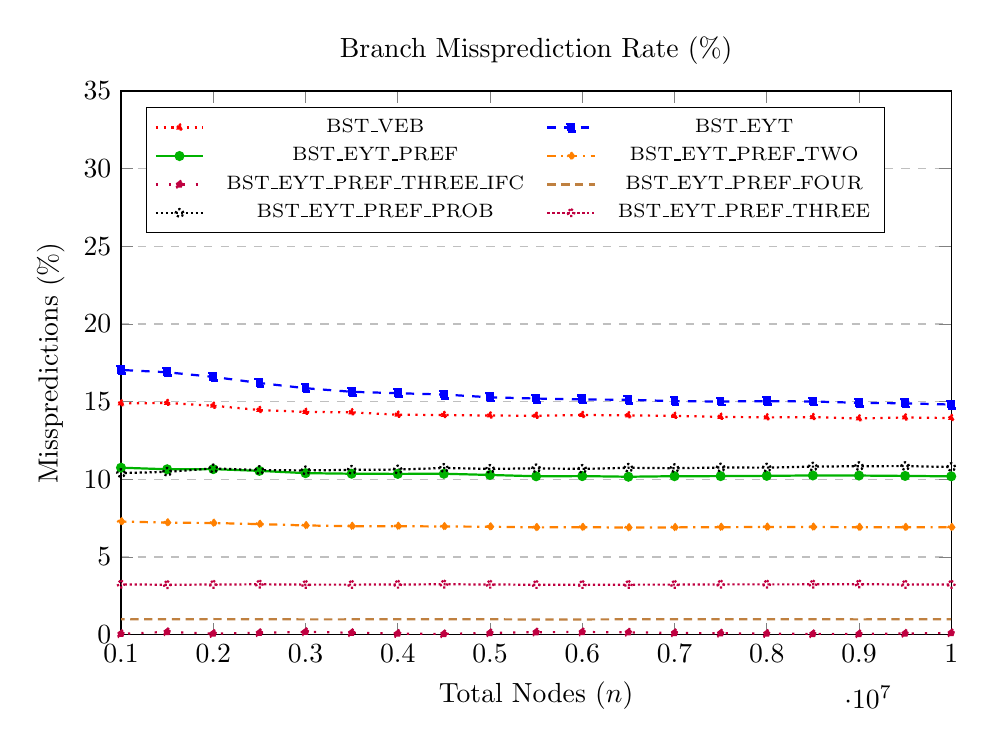
\begin{tikzpicture}
    \begin{axis}[
        title={Branch Missprediction Rate (\%)},
        xlabel={Total Nodes ($n$)},
        ylabel={Misspredictions (\%)},
        width=\textwidth,
        height=0.7\textwidth,
        xmin=1000000, xmax=10000000,
        ymin=0, ymax=35,
        ymajorgrids,
        grid style=dashed,
        legend columns=2,
        legend pos=north west,
        legend style={font=\scriptsize, column sep=6pt},
    ]

\addplot+[red, thick, dotted, mark=triangle*, mark options={scale=.7,fill=red}]
  coordinates {
    (500000,14.9051)
    (1000000,14.886)
    (1500000,14.9183)
    (2000000,14.7399)
    (2500000,14.4635)
    (3000000,14.3419)
    (3500000,14.3132)
    (4000000,14.1602)
    (4500000,14.1416)
    (5000000,14.108)
    (5500000,14.0938)
    (6000000,14.1436)
    (6500000,14.1199)
    (7000000,14.0846)
    (7500000,14.0239)
    (8000000,13.9874)
    (8500000,14.0059)
    (9000000,13.9205)
    (9500000,13.9838)
    (10000000,13.9467)
  };
\addlegendentry{BST\_VEB}

\addplot+[blue, thick, dashed, mark=square*, mark options={scale=.7,fill=blue}]
  coordinates {
    (500000,17.0691)
    (1000000,17.0425)
    (1500000,16.8942)
    (2000000,16.5963)
    (2500000,16.2029)
    (3000000,15.8667)
    (3500000,15.6361)
    (4000000,15.5448)
    (4500000,15.4605)
    (5000000,15.2826)
    (5500000,15.2023)
    (6000000,15.1451)
    (6500000,15.1218)
    (7000000,15.0335)
    (7500000,15.0113)
    (8000000,15.0367)
    (8500000,15.0112)
    (9000000,14.9272)
    (9500000,14.8961)
    (10000000,14.8146)
  };
\addlegendentry{BST\_EYT}

\addplot+[green!70!black, thick, solid, mark=*, mark options={scale=.7,fill=green!70!black}]
  coordinates {
    (500000,10.8029)
    (1000000,10.7508)
    (1500000,10.6499)
    (2000000,10.6598)
    (2500000,10.5474)
    (3000000,10.4004)
    (3500000,10.3635)
    (4000000,10.3526)
    (4500000,10.3619)
    (5000000,10.2841)
    (5500000,10.1997)
    (6000000,10.2098)
    (6500000,10.169)
    (7000000,10.2045)
    (7500000,10.2085)
    (8000000,10.2262)
    (8500000,10.2523)
    (9000000,10.2456)
    (9500000,10.222)
    (10000000,10.1951)
  };
\addlegendentry{BST\_EYT\_PREF}

\addplot+[orange, thick, dashdotted, mark=diamond*, mark options={scale=.7,fill=orange}]
  coordinates {
    (500000,7.34299)
    (1000000,7.28606)
    (1500000,7.21673)
    (2000000,7.19056)
    (2500000,7.12107)
    (3000000,7.03419)
    (3500000,6.98796)
    (4000000,6.98807)
    (4500000,6.96546)
    (5000000,6.95261)
    (5500000,6.90885)
    (6000000,6.92144)
    (6500000,6.89857)
    (7000000,6.9098)
    (7500000,6.9215)
    (8000000,6.9343)
    (8500000,6.9338)
    (9000000,6.91941)
    (9500000,6.91772)
    (10000000,6.91646)
  };
\addlegendentry{BST\_EYT\_PREF\_TWO}

\addplot+[purple, thick, loosely dotted, mark=pentagon*, mark options={scale=.7,fill=purple}]
  coordinates {
    (500000,0.0646867)
    (1000000,0.0619217)
    (1500000,0.182202)
    (2000000,0.073196)
    (2500000,0.121624)
    (3000000,0.187283)
    (3500000,0.122769)
    (4000000,0.0748874)
    (4500000,0.0486832)
    (5000000,0.113432)
    (5500000,0.164708)
    (6000000,0.174774)
    (6500000,0.1528)
    (7000000,0.117215)
    (7500000,0.0932943)
    (8000000,0.0740629)
    (8500000,0.0509059)
    (9000000,0.0505316)
    (9500000,0.0801075)
    (10000000,0.112885)
  };
\addlegendentry{BST\_EYT\_PREF\_THREE\_IFC}

\addplot+[brown, thick, densely dashed, mark=x*, mark options={scale=.7,fill=brown}]
  coordinates {
    (500000,1.00352)
    (1000000,1.0029)
    (1500000,0.989859)
    (2000000,1.00608)
    (2500000,0.996297)
    (3000000,0.988649)
    (3500000,0.990085)
    (4000000,1.00188)
    (4500000,1.00047)
    (5000000,0.992835)
    (5500000,0.983541)
    (6000000,0.986412)
    (6500000,0.991731)
    (7000000,0.993333)
    (7500000,0.991019)
    (8000000,0.993842)
    (8500000,0.996572)
    (9000000,0.988877)
    (9500000,0.994935)
    (10000000,0.99642)
  };
\addlegendentry{BST\_EYT\_PREF\_FOUR}

\addplot+[black, thick, densely dotted, mark=o, mark options={scale=.7,fill=black}]
  coordinates {
    (500000,10.2223)
    (1000000,10.4034)
    (1500000,10.4841)
    (2000000,10.7044)
    (2500000,10.5973)
    (3000000,10.5745)
    (3500000,10.6098)
    (4000000,10.6316)
    (4500000,10.7326)
    (5000000,10.6753)
    (5500000,10.7092)
    (6000000,10.6729)
    (6500000,10.7445)
    (7000000,10.7179)
    (7500000,10.7597)
    (8000000,10.7554)
    (8500000,10.8204)
    (9000000,10.8477)
    (9500000,10.8537)
    (10000000,10.795)
  };
\addlegendentry{BST\_EYT\_PREF\_PROB}

\addplot+[purple, thick, densely dotted, mark=pentagon, mark options={scale=.7,fill=purple}]
  coordinates {
    (500000,3.26263)
    (1000000,3.24302)
    (1500000,3.21625)
    (2000000,3.23146)
    (2500000,3.24566)
    (3000000,3.22411)
    (3500000,3.22435)
    (4000000,3.2331)
    (4500000,3.2483)
    (5000000,3.23328)
    (5500000,3.2183)
    (6000000,3.21681)
    (6500000,3.22403)
    (7000000,3.22464)
    (7500000,3.24162)
    (8000000,3.24181)
    (8500000,3.2428)
    (9000000,3.25367)
    (9500000,3.23145)
    (10000000,3.2317)
  };
\addlegendentry{BST\_EYT\_PREF\_THREE}
    \end{axis}
  \end{tikzpicture}
  \caption[Branch Missprediction Rate]{Branch Missprediction Rate in percent of the different implementations.}
  \label{fig:branchrate}
\end{figure}


\section{Conclusion}
In this project, we implemented and benchmarked different variants of pointer-free binary search trees such as VanEmde-Boas and Eytzinger trees with increasingly aggressive manual data prefetching. We instrumented the program using the \texttt{perf} framework to access metrics such as cache misses and branch mispredictions to evaluate the behavior of the different implementations. We surprisingly encountered the \textit{if-conversion} control-flow optimization of the compiler and included it in our analysis. We found that the Eytzinger-based implementations by default enable the CPU-internal prefetchers to pull in more useful data ahead of time, even without explicit prefetching for up to three levels of the tree. We identified that prefetching beyond three levels likely causes too much contention in the memory system and hence degenerates the performance of the program. We categorized the branches of the different programs into easy and hard-to-predict and found that only the final branch which determines whether to go left or right causes problems to the branch predictor. In fact, the if-converted program uses predicated instructions to virtually eliminate any critical branch misspredition during the execution which results in a significant performance increase compared to the branching variant. 


\newpage
\section{Appendix}
\label{sec:app}
\subsection{\texttt{IBST.h}}
\begin{lstlisting}
#pragma once
#include <cstddef>

template<class Key>
class IBST {
public:
    virtual void insert(const Key& k)                = 0;
    virtual bool contains(const Key& k)        const = 0;
    virtual std::size_t size_bytes()           const = 0;
    virtual ~IBST() = default;
};
\end{lstlisting}
\captionof{lstlisting}[\texttt{IBST.h}]{Abstract interface class for our Binary Search Tree implementationin in \texttt{IBST.h}}
\label{lst:ibst}

\subsection{\texttt{BSTPtr.h}}
\begin{lstlisting}
#pragma once
#include "IBST.h"
#include <memory>
#include <utility>

template<class Key>
class BSTPtr : public IBST<Key> {
    struct Node {
        Key key;
        std::unique_ptr<Node> l, r;
        explicit Node(const Key& k) : key(k) {}
    };

    std::unique_ptr<Node> root_;
    std::size_t node_cnt_ = 0;

    void insertNode(std::unique_ptr<Node>& p, const Key& k) {
        if (!p) {
            p = std::make_unique<Node>(k);
            ++node_cnt_;                         
        } else if (k < p->key) {
            insertNode(p->l, k);
        } else if (k > p->key) {
            insertNode(p->r, k);
        }
    }

    static bool contains(const std::unique_ptr<Node>& p, const Key& k) {
        const Node* cur = p.get();
        while (cur) {
            if (k == cur->key) return true;
            cur = (k < cur->key) ? cur->l.get() : cur->r.get();
        }
        return false;
    }

public:
    void insert(const Key& k) override { insertNode(root_, k); }
    bool contains(const Key& k) const override { return contains(root_, k); }

    std::size_t size_bytes() const override { return node_cnt_ * sizeof(Node); }
};
\end{lstlisting}
\captionof{lstlisting}[\texttt{BSTPtr.h}]{Plain Binary Search Tree implementation in \texttt{BSTPtr.h}}
\label{lst:btspointer}

\subsection{\texttt{BSTVEB.h}}
\label{secsec:vb}
\begin{lstlisting}
#pragma once
#include "IBST.h"
#include <vector>
#include <algorithm>
#include <stdexcept>


namespace help {
template<class Key>
void build_veb(std::vector<Key>& out,
               const std::vector<Key>& sorted, std::size_t lo, std::size_t hi)
{
    if (lo >= hi) return;                       
    std::size_t mid = (lo + hi) / 2;            
    out.push_back(sorted[mid]);                 
    build_veb(out, sorted, lo, mid);            
    build_veb(out, sorted, mid + 1, hi);        
}
} 

template<class Key>
class BSTVEB : public IBST<Key> {
    std::vector<Key> a_;            
    bool              frozen_ = false;
    std::vector<Key>  inserts_;     


    void freeze() {
        if (frozen_) return;

        std::sort(inserts_.begin(), inserts_.end());
        inserts_.erase(std::unique(inserts_.begin(), inserts_.end()),
                       inserts_.end());

        a_.reserve(inserts_.size());
        help::build_veb(a_, inserts_, 0, inserts_.size());
        frozen_ = true;
    }

    bool containsRec(const Key& k,
                     std::size_t lo, std::size_t hi, std::size_t idx) const
    {
        if (lo >= hi) return false;            

        const Key& key = a_[idx];
        if (k == key) return true;

        std::size_t mid        = (lo + hi) / 2;
        std::size_t left_size  = mid - lo;    
        std::size_t left_idx   = idx + 1;   
        std::size_t right_idx  = idx + 1 + left_size;

        return (k < key)
             ? containsRec(k, lo, mid,           left_idx)
             : containsRec(k, mid + 1, hi,       right_idx);
    }

public:
    void insert(const Key& k) override {
        if (frozen_)
            throw std::logic_error("I am already frozen!");
        inserts_.push_back(k);
    }

    bool contains(const Key& k) const override {
        const_cast<BSTVEB*>(this)->freeze();   
        return containsRec(k, 0, a_.size(), 0);
    }

     std::size_t size_bytes() const override { return a_.size() * sizeof(Key); }
};

\end{lstlisting}
\captionof{lstlisting}[\texttt{BSTVEB.h}]{Van Emde-Boas Tree Implementation in \texttt{BSTVEB.h}}
\label{lst:btsvb}

\subsection{\texttt{benchmark.cpp}}
\label{secsec:bcpp}
\begin{lstlisting}
#include "IBST.h"
#include "BSTPtr.h"
#include "BSTVEB.h"
#include "PerfCounters.h"

#include <vector>
#include <random>
#include <iostream>
#include <iomanip>
#include <fstream>
#include "util/json.hpp"
#include <functional>
#include <chrono>

using json  = nlohmann::json;
using Clock = std::chrono::steady_clock;

struct Metrics {
    long long ns          = 0;
    long long ops         = 0;
    long long cache_refs  = 0;
    long long cache_miss  = 0;
};

template<class Key>
Metrics benchOnce(IBST<Key>& tree,
                  const std::vector<Key>& lookups,
                  const std::vector<Key>& inserts)
{
    for (const auto& k : inserts) tree.insert(k);

    PerfCounters pc;
    pc.start();

    auto start = Clock::now();
    for (const auto& k : lookups)
        (void)tree.contains(k);
    auto end   = Clock::now();

    pc.stop();

    Metrics m;
    m.ns         = std::chrono::duration_cast<std::chrono::nanoseconds>(end - start).count();
    m.ops        = lookups.size();
    m.cache_refs = pc.refs();
    m.cache_miss = pc.misses();
    return m;
}

using Factory = std::function<std::unique_ptr<IBST<int>>(void)>;
struct Variant { std::string name; Factory make; };

const std::vector<Variant> variants = {
    {"BST_PTR", [] { return std::make_unique<BSTPtr<int>>(); }},
    {"BST_VEB", [] { return std::make_unique<BSTVEB<int>>(); }},
};

void runExperiment(int n, int q, int T, bool csv,
                   const Factory& make, unsigned seed,
                   const std::string& impl)
{
    std::mt19937 rng(seed);
    std::uniform_int_distribution<int> dist(1, n * 10);

    std::vector<int> inserts(n);
    for (int& x : inserts) x = dist(rng);

    std::vector<int> lookups(q);
    for (int& x : lookups) x = dist(rng);

    long long  acc_ns   = 0;
    long long  acc_refs = 0, acc_miss = 0;
    std::size_t bytes_used = 0;

    for (int t = 0; t < T; ++t) {
        auto tree = make();
        Metrics m = benchOnce(*tree, lookups, inserts);
        acc_ns   += m.ns;
        acc_refs += m.cache_refs;
        acc_miss += m.cache_miss;
        if (t == 0) bytes_used = tree->size_bytes();  
    }

    double avg_ns      = double(acc_ns)   / T;
    double ns_per_op   = avg_ns / q;

    double avg_refs    = double(acc_refs) / T;
    double avg_miss    = double(acc_miss) / T;
    double miss_per_op = avg_miss / q;
    double miss_rate   = (avg_refs > 0) ? avg_miss / avg_refs : 0.0;  
    double avg_s       = avg_ns / 1e9;
    double bytes_mb    = bytes_used / 1024.0 / 1024.0;

    if (csv) {
        std::cout << impl << ','
                  << n << ',' << q << ','
                  << avg_ns << ','
                  << std::fixed << std::setprecision(2)
                  << avg_s << ','
                  << std::defaultfloat
                  << ns_per_op << ','
                  << avg_refs << ',' << avg_miss << ','
                  << miss_per_op << ','
                  << miss_rate << ','
                  << bytes_used  << '\n';
    } else {
        std::cout << std::fixed << std::setprecision(2)
                  << std::left
                  << std::setw(10) << impl
                  << std::setw(10) << n
                  << std::setw(10) << q
                  << std::setw(15) << avg_ns
                  << std::setw(10) << avg_s
                  << std::defaultfloat << std::setprecision(6)
                  << std::setw(15) << ns_per_op
                  << std::setw(15) << avg_refs
                  << std::setw(15) << avg_miss
                  << std::setw(12) << miss_per_op
                  << std::setw(10) << std::fixed << std::setprecision(3) << miss_rate
                  << std::setw(12) << std::fixed << std::setprecision(1) << bytes_mb
                  << '\n';
    }
}

int main(int argc, char* argv[])
{
    int         n    = 10000;
    int         q    = 10000;
    int         T    = 1;
    bool        csv  = false;
    unsigned    seed = 42;
    std::string impl = "ALL";

    if (argc >= 2) {
        std::ifstream in(argv[1]);
        if (!in) { std::cerr << "Cannot open " << argv[1] << '\n'; return 1; }
        json cfg; in >> cfg;
        if (cfg.contains("n"))    n    = cfg["n"];
        if (cfg.contains("q"))    q    = cfg["q"];
        if (cfg.contains("T"))    T    = cfg["T"];
        if (cfg.contains("csv"))  csv  = cfg["csv"];
        if (cfg.contains("seed")) seed = cfg["seed"];
        if (cfg.contains("impl")) impl = cfg["impl"];
    }

    if (argc == 3) impl = argv[2];

    if (!csv) {
        std::cout << std::left
                  << std::setw(10) << "impl"
                  << std::setw(10) << "n"
                  << std::setw(10) << "q"
                  << std::setw(15) << "total_ns"
                  << std::setw(10) << "total_s"
                  << std::setw(15) << "ns/search"
                  << std::setw(15) << "cache_refs"
                  << std::setw(15) << "cache_miss"
                  << std::setw(12) << "miss/search"
                  << std::setw(10) << "missRate"
                  << std::setw(12) << "bytes(MB)" << '\n'
                  << std::string(134, '-') << '\n';
    } else {
        std::cout << "impl,n,q,total_ns,total_s,ns_per_search,"
                     "cache_refs,cache_misses,misses_per_search,miss_rate,bytes\n";
    }

    for (const auto& v : variants) {
        if (impl != "ALL" && impl != v.name) continue;
        runExperiment(n, q, T, csv, v.make, seed, v.name);
    }
    return 0;
}

\end{lstlisting}
\captionof{lstlisting}[\texttt{BSTVEB.h}]{Benchmarking Driver in \texttt{benchmark.cpp}}
\label{lst:benchcpp}

\subsection{\texttt{PerfCounters.h}}
\label{secsec:perfsetup}
\begin{lstlisting}
#pragma once
#include <linux/perf_event.h>
#include <cstdint>         
#include <sys/syscall.h>    
#ifndef __NR_perf_event_open
#endif
#include <sys/ioctl.h>
#include <unistd.h>
#include <cstring>
#include <cerrno>
#include <stdexcept>
#include <array>

class PerfCounters {
    int fd_refs_{-1}, fd_misses_{-1};
    long long refs_{0}, misses_{0};

    static int openCounter(uint32_t type, uint64_t config)
    {
        perf_event_attr pea{};
        pea.type           = type;
        pea.size           = sizeof(perf_event_attr);
        pea.config         = config;
        pea.inherit        = 0;       
        pea.disabled       = 1;
        pea.exclude_kernel = 0;
        pea.exclude_hv     = 1;

        int fd = syscall(__NR_perf_event_open, &pea, 0, -1, -1, 0);
        if (fd == -1)
            throw std::runtime_error{"perf_event_open: " + std::string(strerror(errno))};
        return fd;
    }
public:
    PerfCounters()
    {
        fd_refs_   = openCounter(PERF_TYPE_HARDWARE, PERF_COUNT_HW_CACHE_REFERENCES);
        fd_misses_ = openCounter(PERF_TYPE_HARDWARE, PERF_COUNT_HW_CACHE_MISSES);
    }
    ~PerfCounters() { close(fd_refs_); close(fd_misses_); }

    inline void start() const { ioctl(fd_refs_, PERF_EVENT_IOC_RESET, 0); ioctl(fd_misses_, PERF_EVENT_IOC_RESET, 0);
                                ioctl(fd_refs_, PERF_EVENT_IOC_ENABLE, 0); ioctl(fd_misses_, PERF_EVENT_IOC_ENABLE, 0); }
    inline void stop()
{
    ioctl(fd_refs_,   PERF_EVENT_IOC_DISABLE, 0);
    ioctl(fd_misses_, PERF_EVENT_IOC_DISABLE, 0);

    if (read(fd_refs_, &refs_, sizeof(refs_))   != sizeof(refs_))
        throw std::runtime_error("failed to read cache-refs counter");
    if (read(fd_misses_, &misses_, sizeof(misses_)) != sizeof(misses_))
        throw std::runtime_error("failed to read cache-miss counter");
}
    long long refs()   const { return refs_;   }
    long long misses() const { return misses_; }
};

\end{lstlisting}
\captionof{lstlisting}[\texttt{PerfCounters.h}]{Instrumentation Setup for Perf in \texttt{PerfCounters.h}}
\label{lst:perfsetup}


\subsection{\texttt{small.json}}
\label{secsec:smalinstance}
\begin{lstlisting}
{
  "n"   : 100000,
  "q"   : 100000,
  "T"   : 5,
  "csv" : false,
  "seed": 123
}
\end{lstlisting}
\captionof{lstlisting}[\texttt{small.json}]{Example Instance in \texttt{small.json}}
\label{lst:exampleinstance}

\newpage
\printbibliography

\end{document}
